%\addcontentsline{toc}{chapter}{Software}
\chapter{Software}

 %%%%%%% INTRODUCTION %%%%%%
%%\addcontentsline{toc}{section}{Introduction}
%\section{Introduction}
In this section the software developed in this Bachelor's Thesis is presented and thoroughly explained. 
\\

The code was created as a ROS package. ROS (Robotic Operating System) is an Operating System designed to be implemented in robots. It has libraries to enhance the communication between nodes, the processes management or the threads present in the code among other functionalities. 
Since this code is intended to be running on a robot, the software developed was created as a ROS package. 
\\

In order to manage 2D and 3D information (images and pointclouds) two libraries has been used: OpenCV, and PCL. Those two libraries implement basic and state-of-the-art algorithms that allow a easier and more time-efficient management of the data. Further information about these libraries might be found on the sections \ref{opencv} and \ref{pcl} respectively. 
\\

The software was structured in nodes. These nodes have a relatively small functionality and run in parallel. The fact that they run simultaneously improves the efficiency of the code lowering the lag due to time-expensive operations. 
\\

In the following sections, the software structure and tools used are described. 
%%%%%%% TOOLS %%%%%%
%\addcontentsline{toc}{subsection}{Tools}
\section{Technologies}
\label{technologies}

This section presents the different technologies used in the development of this thesis. It was previously mentioned that the whole code constitutes a ROS package, and that it uses the OpenCV and PCL libraries. 
\\

In the following sections these technologies are described and its use withing the code explained. 

\section{ROS}
\label{ros}

ROS is the acronym of Robot Operating System\cite{ros}. It is an open source set of libraries and various tools that are aimed at robot applications. It is intended as well to improve the efficacy of collaborative robotics development, allowing easy interconnection of ROS packages. 


\begin{figure}[h]
	\begin{center}
    
\includegraphics[scale=0.3]{img/ros/groovy.eps}
	\caption[ROS Groovy Logo]{ROS Groovy Logo}
	\end{center}
\end{figure}

The tools, libraries and third-party packages available in the different ROS distributions are very useful when programming software for a robot. This is the main reason why this Operating System was selected as the framework in which develop the code of this Bachelor's Thesis. 
\\

The structure of the software is detailed in the chapter \ref{software_structure}.  It is a node structure in which different processes are executed in parallel in order to improve the efficiency of the code. Each node executes a different computation in the data-flow. 
\\

Since each node is part of a chain of information between the input and output of the system, they must be connected. This information sharing is produced using the ROS topics. 


The ROS nodes are simply executables that uses the ROS messaging system to communicate with other nodes. The ROS topics are a messaging units in which the nodes can publish messages. Also, the nodes may subscribe to those topics in order to retrieve the messages already published on them. 
\\

The messages are pieces of data that the nodes send to each other. In ROS, the messages might be customized combining the already defined standard messages and sensor messages to create the message with the information needed. In this project various custom messages has been defined. More information about those can be found in the \ref{software_messages} section. 



\newpage

\subsection{OpenCV}
\label{opencv}

%Intro
OpenCV\cite{opencv} (Open Source Computer Vision) is a library that implements state of the art real-time computer vision 
algorithms. 

It is cross-platform and it is released under a BSD\cite{BSD} license. Previously it was integrated in ROS \cite{ros}, but
now it is used as a stand-alone library.  

\begin{figure}[h]
	\begin{center}
    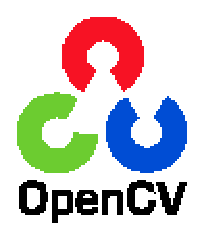
\includegraphics[scale=1]{img/opencv/logo.eps}
	\caption[OpenCV Logo]{OpenCV Logo}
	\end{center}
\end{figure}

The qualities described above as well as its optimization of various algorithms make this library an extremely useful 
asset for robotic vision projects. 

% In this project's context

In this project the C++ interface of the OpenCV library has been used. The functionalities provided by this library are used in all the 2D information management. The next paragraph details the operations for which this library has been used. 

\subsubsection{Processes that use the OpenCV library}

\begin{itemize}
	\item\textbf{Segmentation of the ROI (Region Of Interest)\\ }

	This library allows to crop the original raw image coming
	from the RGB-D sensor. In this application, the region cropped is the one around the hand being used. More information about this operation can be found in the \ref{roi_segmenter_2d} section. 
	

	\item {Keypoints and descriptors extraction\\ }
	 The OpenCV library implements multiple optimized state of the art algorithms. Among them, there are a number of descriptor extractors such as SIFT, SURF, ORB. This last one is being used in this project due to its open-sourceness, and robustness / speed relation. More information about the different algorithms implemented in OpenCV used to extract the descriptors can be found in the section \ref{features}.


	\item {Descriptors matching\\ } There are many different matchers that might be used. In this project, a FlannBasedMatcher
	is being used for this purpose. 
\end{itemize}



\subsubsection{Features}
\label{features}
In this section the most important algorithms regarding object learning and recognition and joint detection and tracking related to this bachelor's thesis are going to be presented.

The most used algorithms due to their relation between performance, invariantness and speed are exposed below. They are presented chronologically and the differences, similarities and improvements between them are explained. 
\\

The selection of one algorithm or another depends on the requisites and the hardware of the application.
\\

These first algorithms, SIFT, SURF and ORB are used to obtain descriptors for 2D data. 

		%\addcontentsline{toc}{subsection}{SIFT}
\subsection{SIFT}

SIFT (Scale Invariant Feature Transform) is a scale and rotation invariant feature descriptor\cite{sift}. 

There are various papers in which the performance of SIFT is compared with other descriptors, such as \cite{Mikolajczyk2005}. In them, it can be seen that SIFT outperforms the others, mainly due to its combination of local information and relative strengths and orientations of gradients. This combination makes it more robust to illumination and viewpoint changes and the addition of noise. 
\\

In order to minimize the cost of extracting such a distinctive features, a cascade filtering approach is used in order to apply the most time-consuming operations only at locations that pass an initial test. 
\\

Its relation between distinctiveness and speed is good. It can be used for on-line applications but it still has a latency that could be improved. Hence, it is an almost real-time algorithms. As an example, in \cite{sift_fpga} the SIFT algorithm was implemented on a FPGA (Field Programmable Gate Array), improving its speed by an order of magnitude and thus allowing it to run in real-time.
\\

The main reason of this high computing time, which is acceptable for on-line applications but improvable, is the descriptor vector size. In the aim of creating a highly distinctive descriptor, the vector is over-dimensioned slowing the detection, description and matching processes. 
\\

In relation with object recognition, this algorithm has a good performance in medium cluttered spaces. If the image is cluttered, there will appear a number of features of the background that do not have a match in the given database. Hence, it will give false positives and the match will have a lower probability. 


		\addcontentsline{toc}{subsection}{SURF}
\subsection*{SURF}
SURF(Speeded Up Robust Features) is a scale and rotation invariant interest point detector and descriptor \cite{surf}. 
It is a proprietary algorithm that simplifies the detection, extraction of the descriptors and matching steps thus obtaining them much faster than previous algorithms without losing repeatability, distinctiveness or robustness. 
\\

The first step of the algorithm is to identify the interest points such as corners, blobs or T-junctions. As it can be seen, this algorithm will be useful when evaluating a textured object. 
\\

The next step is to represent the neighbourhood of the interest points as a feature vector. 
\\

The final step is to match the descriptor vectors between different images, in order to stablish a recognition of a pattern. Usually the matching is performed using as a reference the distance between the vectors. 
In this part, it can be perceived that the size of the descriptor vectors affects directly the performance of the algorithm. SIFT aims to reduce that size without losing distinctiveness in the features. 
\\

The SURF algorithm appeared after SIFT and hence it is interesting to see the similarities and differences between the two. In the previous chapter it was seen the good results obtained when combining the local information and relative data regarding gradients. This algorithm is based on similar characteristics: 
First, an orientation based on the information extracted from a circular region with the interest point as its center is obtained. Then, a square region aligned to that orientation is described and the descriptor is extracted from it.  
\\

From the experiments in \cite{surf} it can be seen that the performance of this descriptors equals and in some cases improves the one of the SIFT descriptors. Also, the SURF descriptors are much faster computed and matched. 



		%\addcontentsline{toc}{subsection}{ORB}
\subsection{ORB}
ORB (Oriented FAST and Rotated BRIEF) is a fast rotation invariant, noise resistant binary descriptor based on BRIEF \cite{orb}.
It is claimed in its presentation paper that it is two orders of magnitude faster than SIFT while matching its performance in many situations. As it can be seen, since ORB is not scale invariant, if the scale difference is noticeable the SURF algorithm will outperform ORB. 
\\

The features used in ORB builds on the FAST\cite{fast} keypoint detector and the BRIEF\cite{brief} descriptor. Both of this previous algorithms offer a good performance and computing time relation. Since neither of them had the orientation taken into account, the main improvement made by the ORB developers is to include this feature in the algorithms. Also, the computation of oriented BRIEF features was improved and an analysis of variance and correlation for this features created. 
\\

FAST is mainly used to find keypoints in real-time systems that match visual features. The orientation operator included in this algorithm is the centroid operator described in \cite{orientation_corners}. This technique is not computationally demanding and also, unlike SIFT, it returns a single dominant result. 
\\

BRIEF uses simple binary tests whose performance is similar to SIFT with regard to robustness to lighting, blur and perspective distortion, but it is sensitive to in-plane rotation. In order to eliminate this drawback, the lowest computing costing solution is to steer BRIEF accordingly with the orientation of the keypoints. 
\\

In the different tests in \cite{orb} can be seen that the percentage of inliers obtained with ORB are higher and do not variate as much as those obtained by SIFT or SURF. 
ORB is then a good alternative for the latter if the application does not need a scale invariant descriptor. 
\\

Finally, it is noticeable that this algorithm is Open Source, since the previous ones are proprietary. 








\section{PCL}


\subsection{Point Cloud}
A point cloud is a data structure that represents a set of multi-dimensional points that is used to represent three-dimensional data. There are two types of point clouds: 3D point cloud in which the points represent the x, y and z coordinates and that has no color information and 4D point cloud in which the color information is included. 
\\

Point clouds are acquired from hardware sensors such as RGB-D sensors, 3D scanners or time-of-flight cameras. Also, those data structures might be generated synthetically. PCL can process data from devices such as the PrimeSensor 3D cameras, the Microsoft Kinect or the Ausus XTionPRO.









\newpage

\subsection{Solution description}

The input of the system is the information coming from the RGB-D sensor. There are two different data that are taken: the 2D information, i.e. the raw image detected by the sensor's camera, and the 3D information, i.e. the raw point cloud. Also, there is another input to the system that shows the position of the different user's joints. This data is provided by a third-party package called pi\_tracker that is explained in the following chapters. 
\\

The software was designed to be running on a robot as was previously explained. This implies that there can not be a GUI (Graphical User Interface) on a screen because the robot being used might not have it. Also, the usability and easiness to learn how to interact with the program was important to allow different people not only investigators to use it. 
\\


\begin{figure}[H]
	\begin{center}
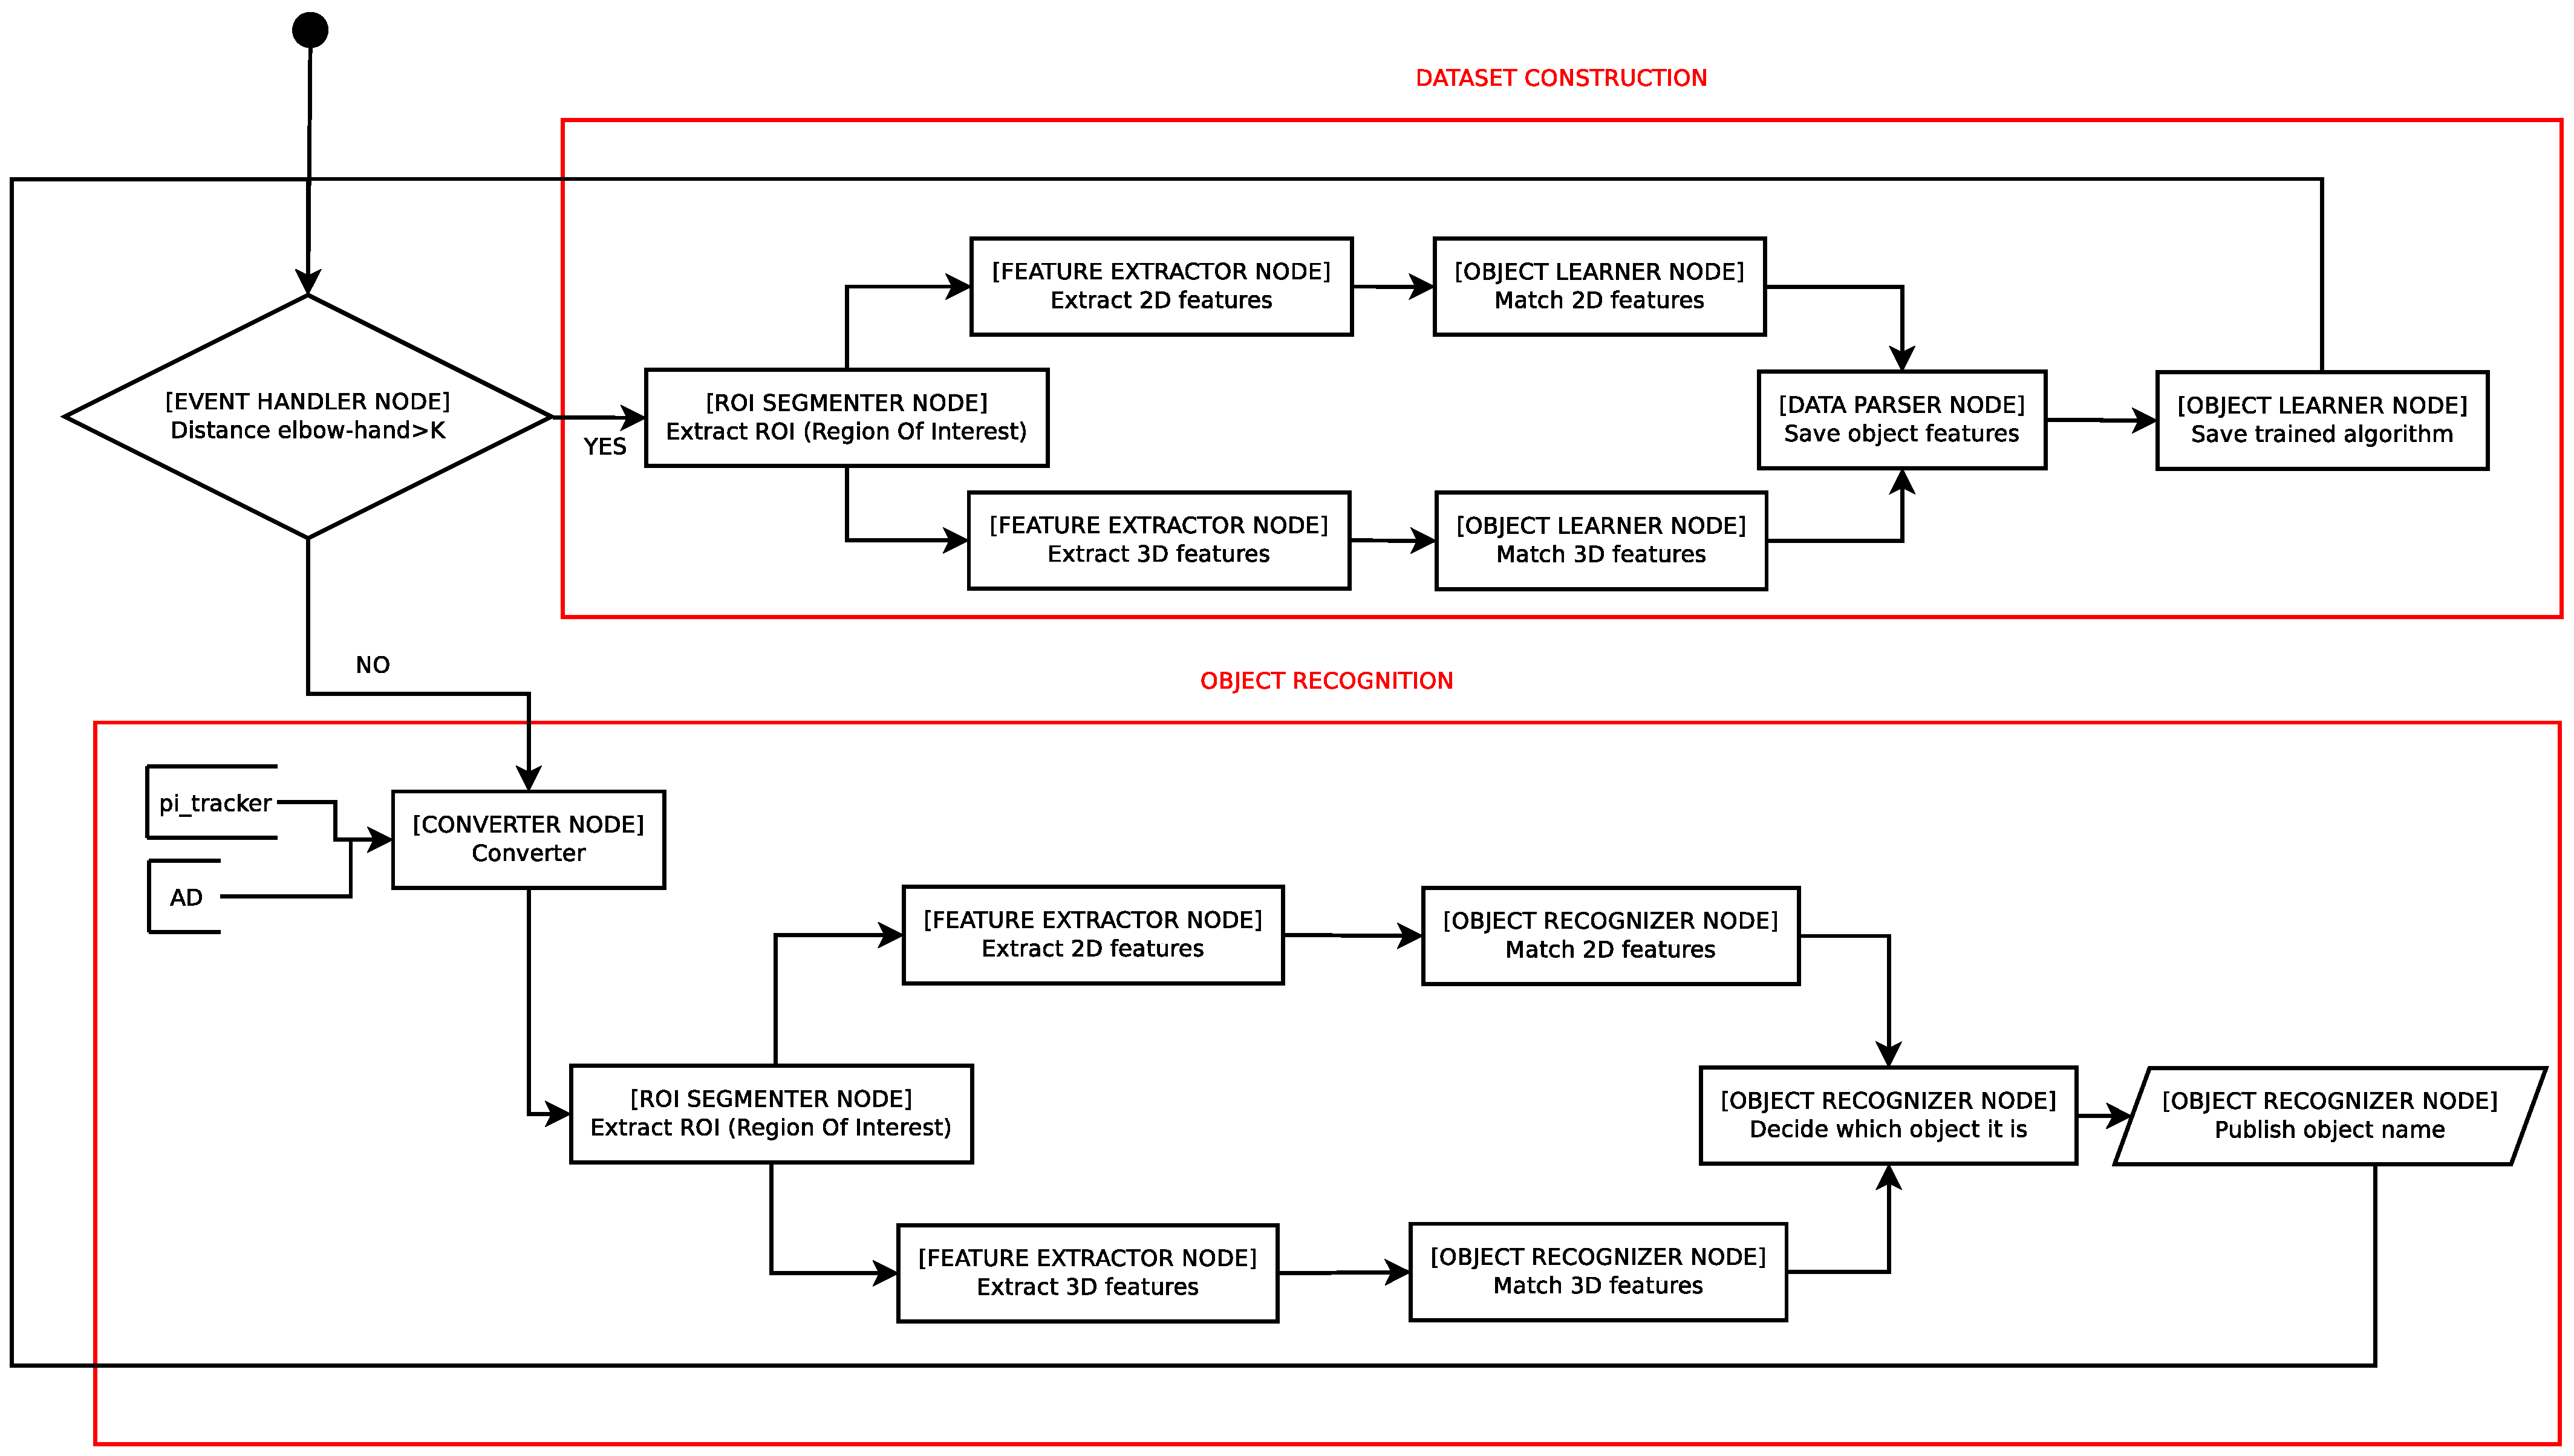
\includegraphics[scale=0.3]{img/diagrams/flowcharts.eps}
	\caption[Software flowchart]{Complete Software flowchart showing the different processing steps between the input and the output}
	\end{center}
\end{figure}


In order to fulfill those requirements a gestural interface was designed. It is developed by a separate node so the processing lags will not affect the recognition of the different gestures. This fact also allows an easy change of the gestures being used. 
\\

The recognition of the location of the hand with respect to the user's body shows how the arm is positioned. If it is stretched towards the sensor, the software enters the dataset construction mode, i.e. the data acquisition and learning mode. If, otherwise, it is located closer to the body, the software starts the object recognition mode. 
\\


The upper part of the diagram shows the data acquisition work-flow. The first step is to extract the ROI (Region of Interest) from the input raw data. This is a crucial step that allows to reduce noticeably the amount of time due to computation reducing the size of the processed information. 
\\

After the extraction, the 2D and 3D features of the segmented data are obtained. The features or descriptors are characteristics that define and represent the data from where they were created. There are different algorithms that perform this task with better or worse repeatability and robustness. All the details about this process is explained in the next chapters. 
\\

That is the end of the data cycle of the learning process. It is iterated over the number of views for each object that is required in order to obtain all the templates necessary per object. 
\\

The recognition mode was triggered when the hand was located near the user's body. This mode can be seen in the lower part of the previous diagram. 
\\

The steps that compose this part of the software are the following: 
First, the input information is converted to the custom message used within the code. Afterwards, as in the previous mode, the Region Of Interest is segmented from both 2D and 3D original information. Then, the descriptors are extracted exactly the same way as in the previous mode. 
\\

The next step is the recognition algorithm. This matches the descriptors from both the image and the point cloud and decides which object of the dataset is more similar to the one that is currently on the user's hand. More details about this algorithm may be found in this section. 
\\

Finally, the object identification number is obtained. This data is the output of the system. 


\newpage
\subsection{Third party libraries that process the input data to the system}
\label{ros_packages}
In this section the ROS packages that are used in our system are presented. 
All of them are used for the initial processing of the data coming from the RGB-D sensor. 
The connection between them and the developed nodes are explained in this section and in section \ref{nodes}.

\subsubsection{ROS package: openni\_camera}
\label{openni_camera}

This package implements the RGB-D sensors drivers.
% It is needed to connect the kinect to the computer. 
% The package is composed of nodes that perform different tasks and publish the results in topics. 
% As an example, a node transforms the raw output information of the kinect into a data array for further processing. 
The package transforms the input raw data coming from the kinect into structured one. 
This information is prepared hence for further processing. 
Figure \ref{diagram_kinect_data} shows the Connectivity graph of this package and its position in the RGB-D sensor data processing chain. 
 
 		\begin{figure}[H]
			\begin{center}
			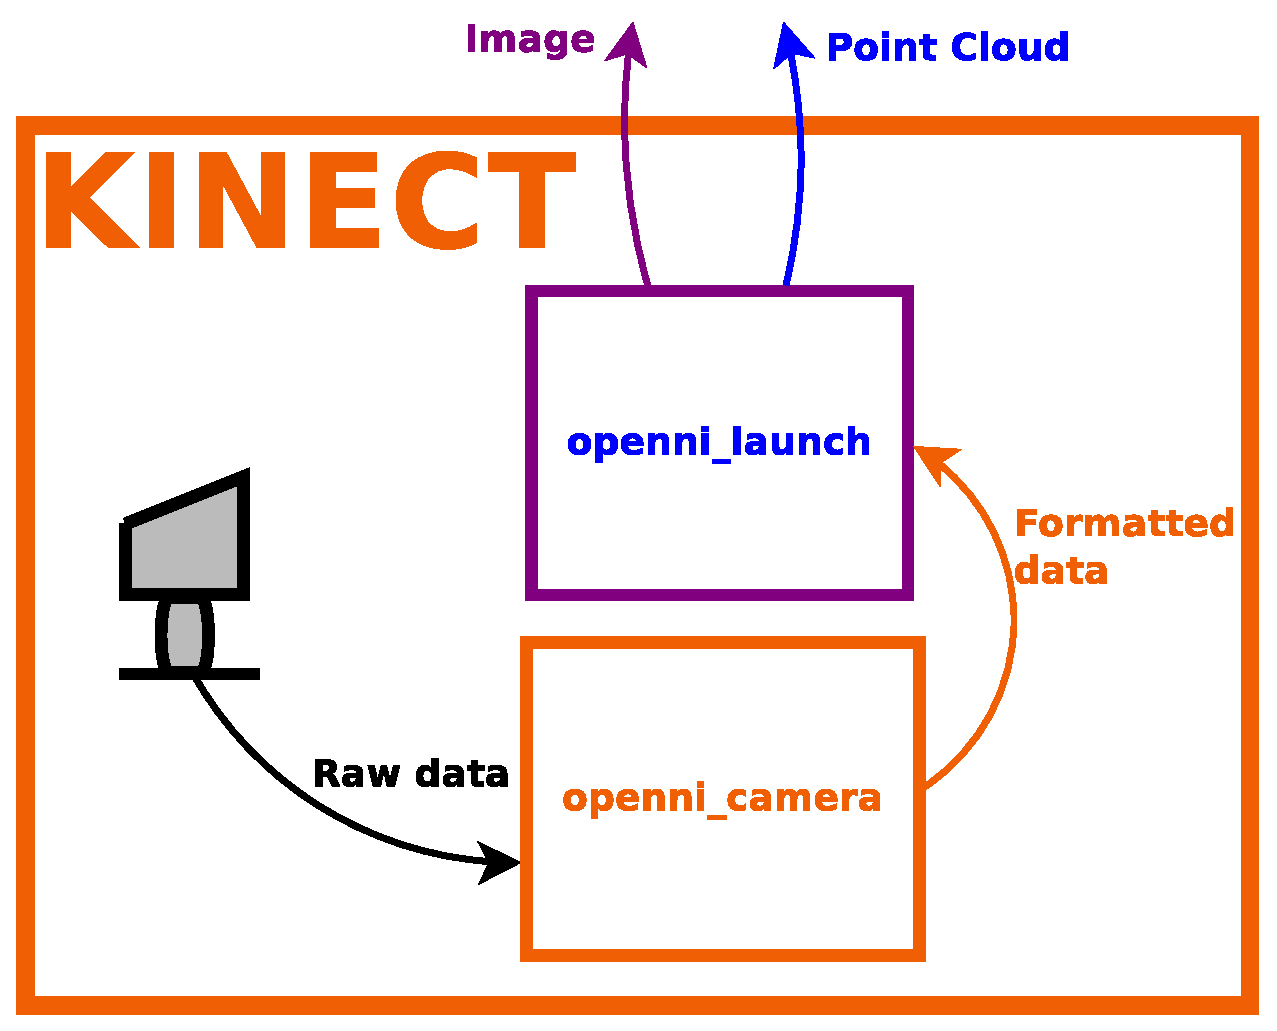
\includegraphics[width=0.5\linewidth]{img/diagrams/kinect_data.eps}
			\caption[Kinect data processing]{Kinect data processing using the openni ROS packages (openni\_camera and openni\_launch).}
			\label{diagram_kinect_data}
			\end{center}
		\end{figure}


\subsubsection{ROS package: openni\_launch}
\label{openni_launch}

This package provides useful transformations taking as input the openni\_camera topics. %and a launch file that executes nodelets with that information. 
It is composed of various nodes that can be executed using a launch file. 
Each node processes the raw input information from the driver into more useful data. 
This data may be a point cloud with color information or a disparity image for example. 
The output of the nodes is published into different topics. 
% The developed nodes described in section \ref{nodes} are subscribed to these topics in order to obtain the input point cloud and image. 
These topics are the input for the nodes that have been developed for this thesis.

\subsubsection{ROS package: pi\_tracker}

This ROS package implements a joint tracker.
It is used within the system to determine the position and orientation of the user's joints. 
This task is performed by the skeleton tracker node.  
Figure \ref{diagram_skeleton} shows the Connectivity graph of this node. 
% In figure \ref{diagram_skeleton} it may be observed that the diagram presented in figure \ref{diagram_kinect_data} is simplified.  

		\begin{figure}[H]
			\begin{center}
			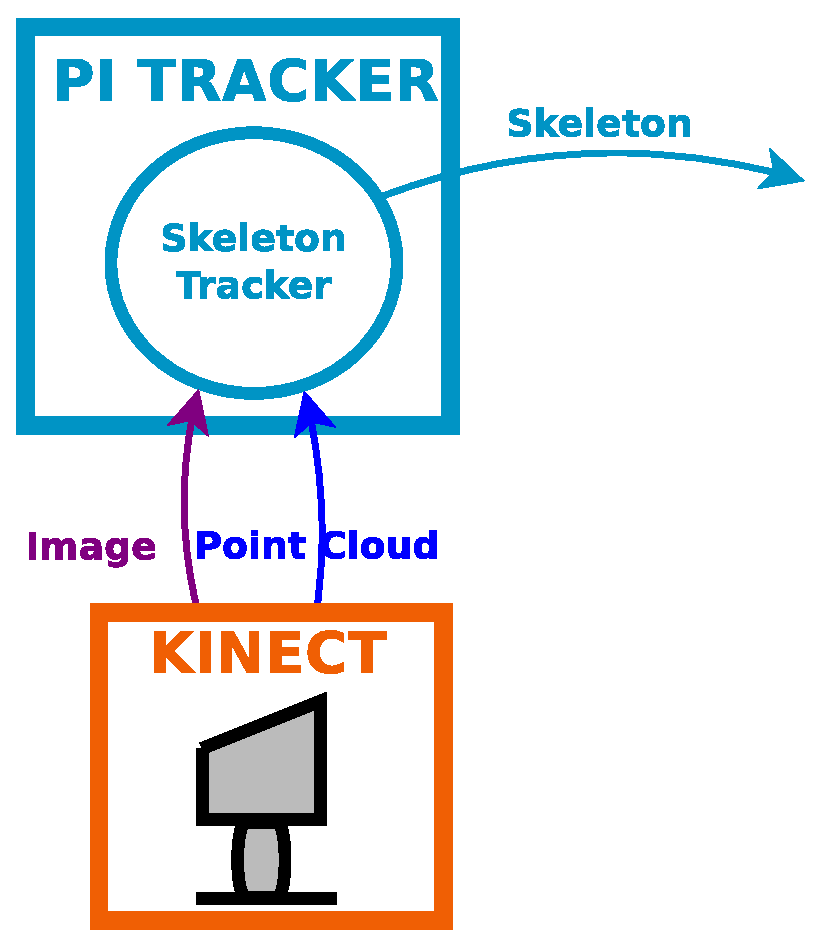
\includegraphics[width=0.3\linewidth]{img/diagrams/node_pi_tracker.eps}
			\caption[Skeleton Tracker I/O]{Connectivity graph of the Skeleton Tracker node.}
			\label{diagram_skeleton}
			\end{center}
		\end{figure}

It can be seen that the node takes as input the output data of the openni\_launch ROS package. 
The node outputs the Skeleton message in which the positions and orientations of the joints are represented. 



%\newpage
%%%%%%% SOFTWARE NODES %%%%%%
%\addcontentsline{toc}{subsection}{Software nodes}
\subsection{Description of the developed nodes}
\label{nodes}


The processing of the system is divided in nodes. 
Figure \ref{nodes_graph} shows the graph of the nodes that have been developed for the project.
% First the ones using the raw input data to the system and afterwards the ones that deliver the output of the system are described.
The circles represent the nodes. %Each circle is a node and the name inside them is the one being used in the software. 
The arrows show the communication between nodes. 
The names next to the nodes' interconnections are the messages interchanged.  % that those processes interchange. 
% The squares with the names serve as separators of the different packages that are being used. 
The square areas define the different ROS packages that have been used.
The square with the tile "OCULAR" separates the nodes developed in this thesis from third-party nodes. 
% All the nodes inside the square with the title "OCULAR" are the ones I developed. 
Sections \ref{converter} to \ref{last_node} present the processing performed by each node. 
\\


		\begin{figure}[H]
			\begin{center}
			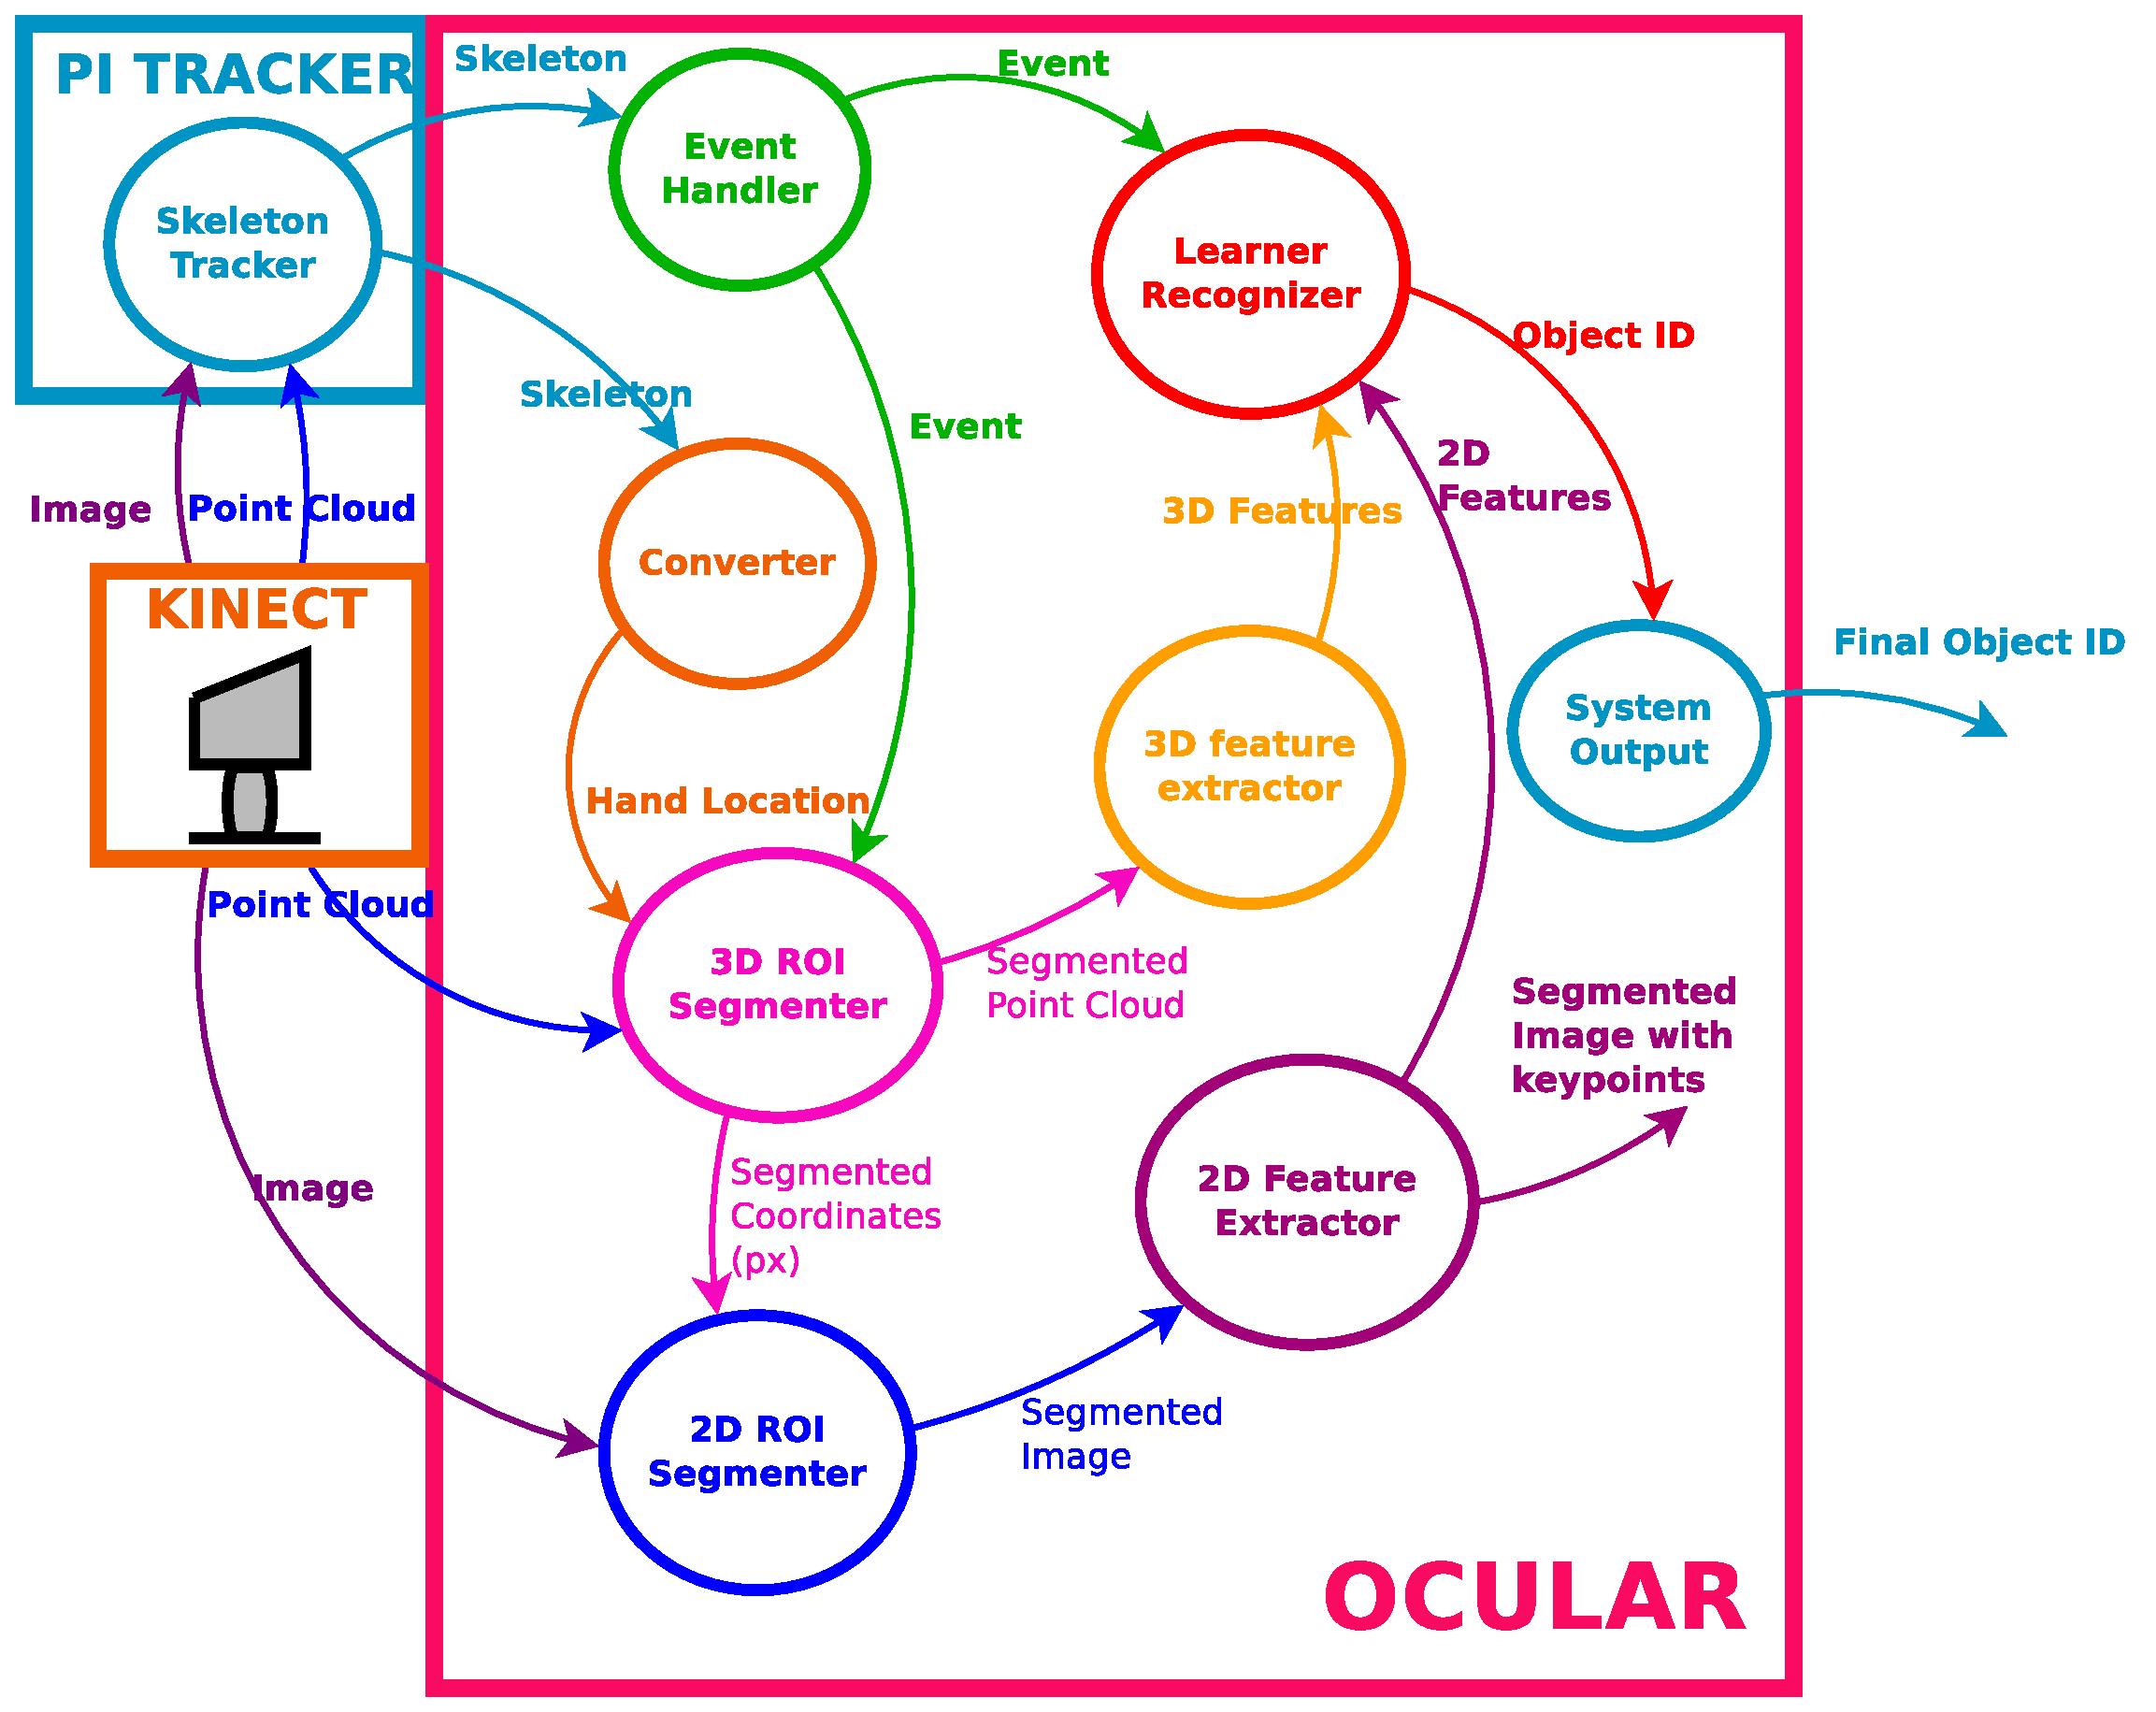
\includegraphics[width=\linewidth]{img/diagrams/nodes.eps}
			\caption[System nodes]{System nodes and their interaction.}
			\label{nodes_graph}

			\end{center}
		\end{figure}

%\newpage



%%\newpage


\subsubsection{Converter node}
		\label{converter}

	This node is the first step of the developed software. 
	It converts the input data containing the skeleton position to a custom message used through the rest of the code. 
	It allows to easily change the package from which the skeleton is obtained without affecting the whole system. 
	The converter node transforms the input data from the pi\_tracker package into the custom message used within the software. 
	It was only implemented a converter for the pi\_tracker package, but it could be easily developed a converter for other packages that retrieve the skeleton position. 
	Figure \ref{node_converter} represents the Connectivity graph of the node. 
	The skeleton message enters the node and the custom message containing the hands location is the output. 

		\begin{figure}[H]
			\begin{center}
			\includegraphics[width=0.5\linewidth]{img/diagrams/node_converter.png}
			\caption[Converter node I/O]{Connectivity graph of the Converter node.}		
			\label{node_converter}
			\end{center}
		\end{figure}

	% The information provided by that third-party code contains the position in the space of each joint of the body. 
	% The converter node takes only both hand's position. 
	The use case diagram of the node can be seen in figure \ref{uc_converter}. 

	\begin{figure}[H]
		\centering
		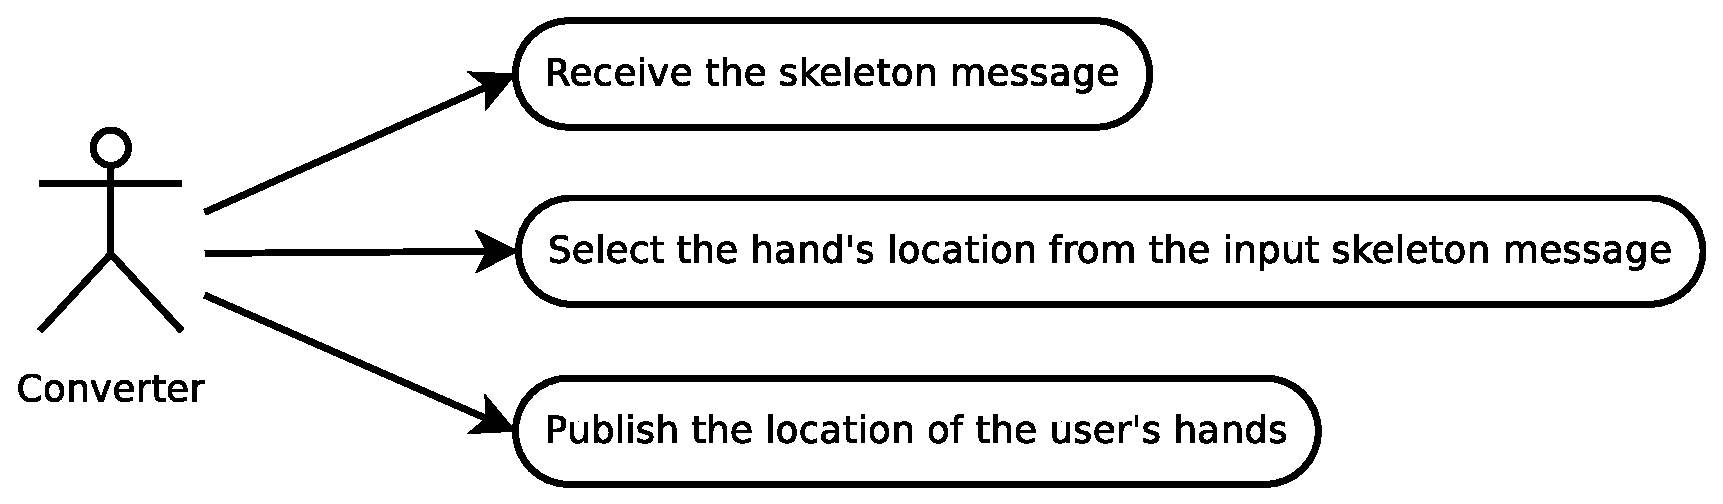
\includegraphics[scale=0.4]{img/diagrams/uc_converter.eps}
		\caption[Use case diagram converter node]{Use Case diagram of the converter node}
		\label{uc_converter}
	\end{figure}

	
	%%\newpage

\subsubsection{3D ROI Segmenter node}
	\label{roi_segmenter_3d}

	Figure  \ref{node_roi3d} presents the Connectivity graph of the node. 
	The input of this node is the raw 3D information from the sensor and the hand's locations from the third-party package pi\_tracker, as well as the hand in which the user is holding the object. 

		\begin{figure}[H]
			\begin{center}
			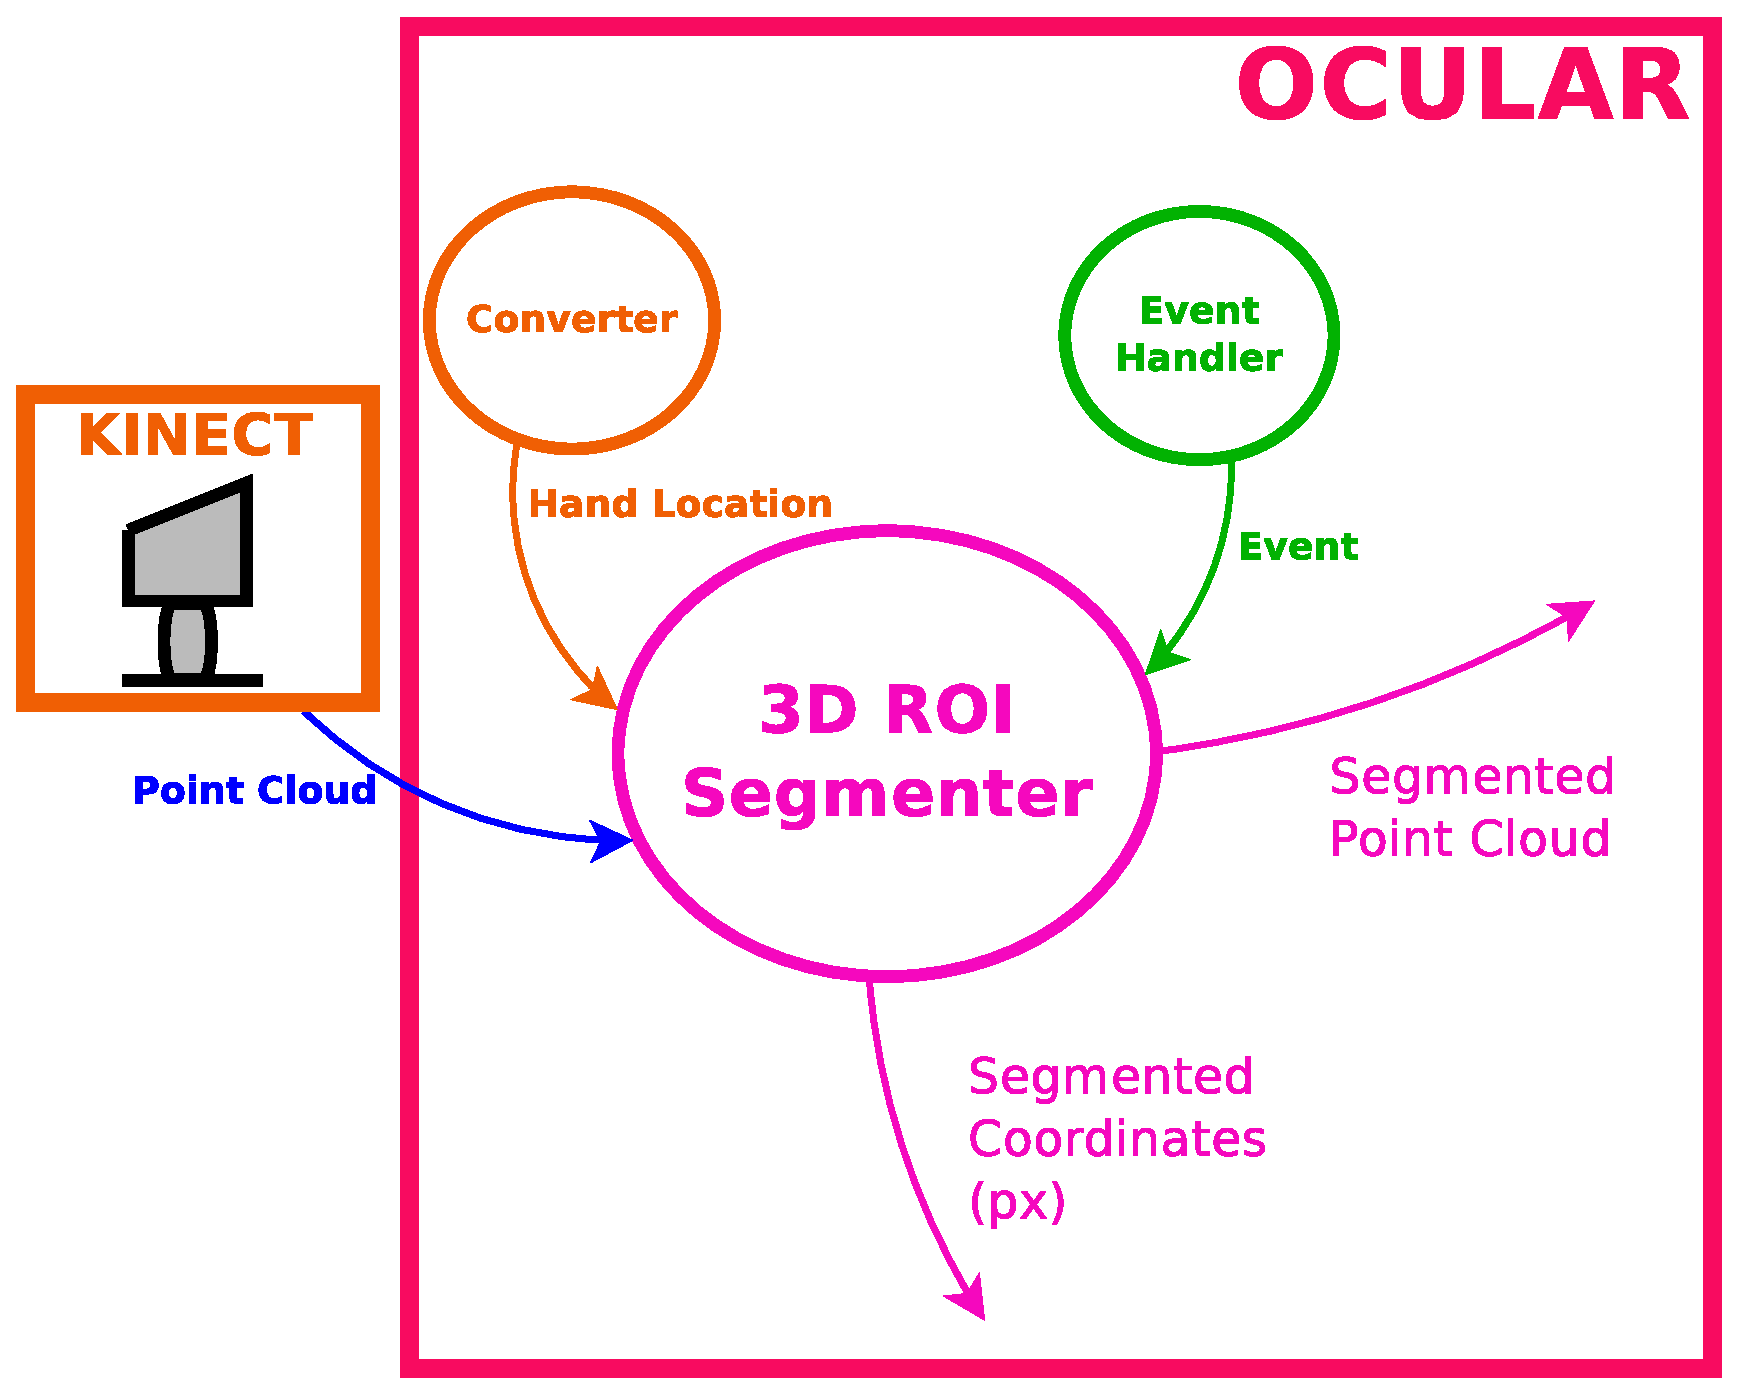
\includegraphics[width=0.5\linewidth]{img/diagrams/node_roi3d.eps}
			\caption[ROI segmenter 3D node I/O]{Connectivity graph of the ROI segmenter 3D node.}		
			\label{node_roi3d}
			\end{center}
		\end{figure}


	The node segments a prism from the original point cloud around the selected hand's center. 
	The prism vertex coordinates are transformed from world coordinates to pixels. 
	This is done to allow the ROI Segmenter 2D to perform the cropping of the input image using those pixel values. 
	That information is the output of the node, together with the segmented point cloud. 
	Figure \ref{uc_roi3d} shows the use case diagram of the node. 

	\begin{figure}[H]
		\centering
	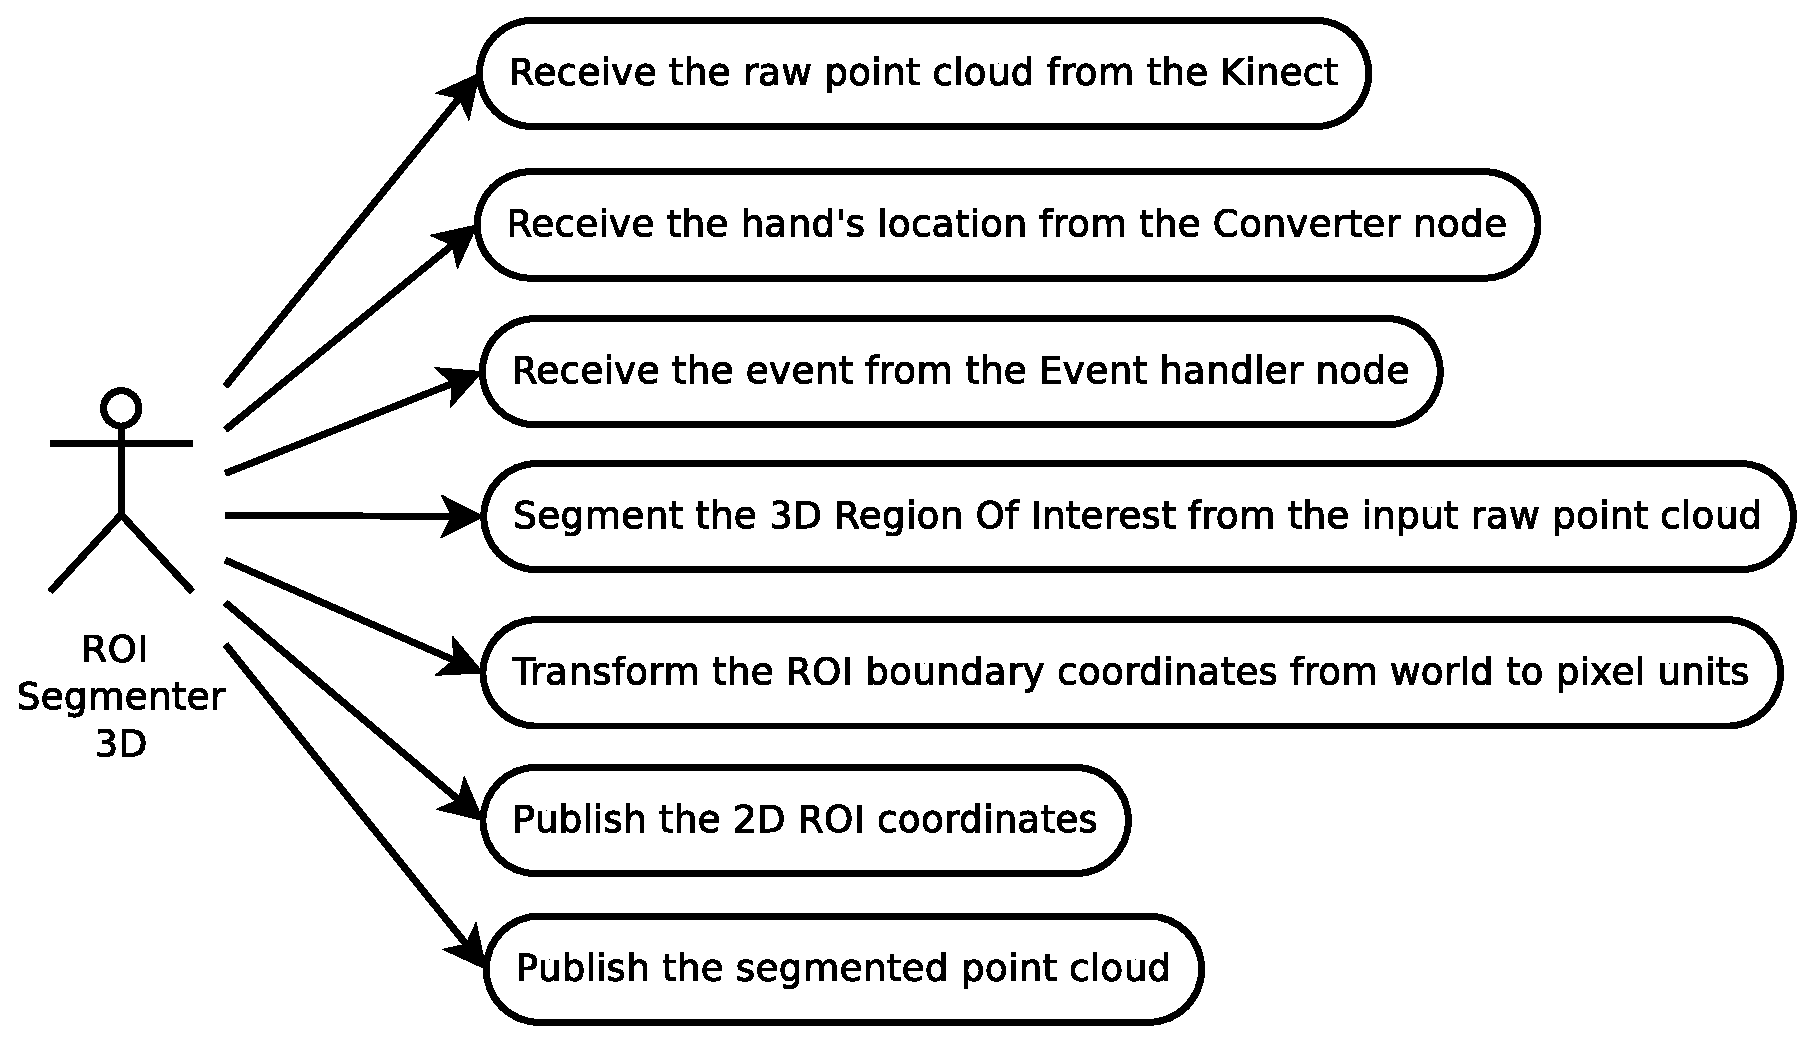
\includegraphics[scale=0.4]{img/diagrams/uc_roi_segmenter_3d.eps}
		\caption[Use case diagram ROI segmenter 3D node]{Use Case diagram of the ROI segmenter 3D node}
		\label{uc_roi3d}	
	\end{figure}
 
%%\newpage

\subsubsection{2D ROI Segmenter node}
	\label{roi_segmenter_2d}
	
	%The present node takes as the input the raw 2D information from the RGB-D sensor and the hand's locations in pixels returned from the ROI segmenter 3D node. 
	Figure \ref{node_roi2d} depicts the Connectivity graph of this node. 
	The raw 2D information and the hand location in pixels are inputs to the ROI Segmenter 2D node. 

		\begin{figure}[H]
			\begin{center}
			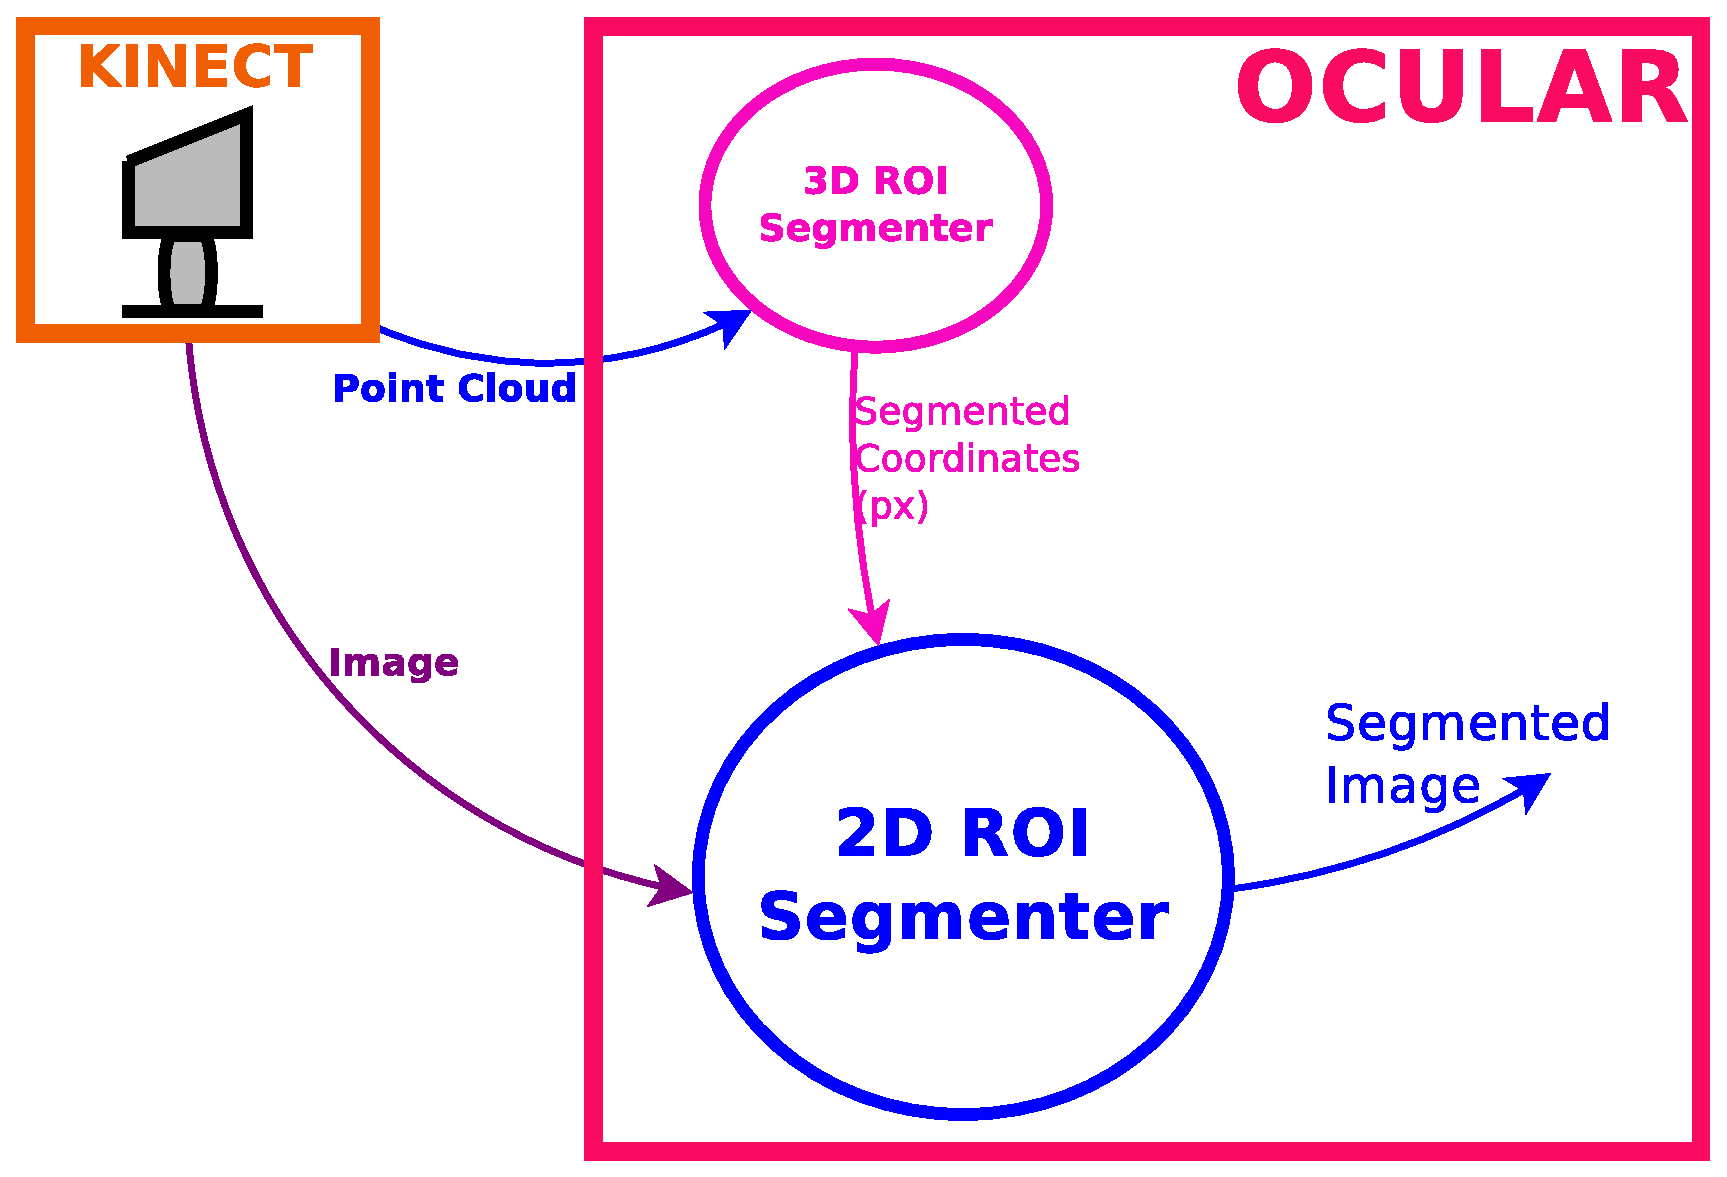
\includegraphics[width=0.5\linewidth]{img/diagrams/node_roi2d.eps}
			\caption[ROI segmenter 2D node I/O]{Connectivity graph of the ROI segmenter 2D node.}		
			\label{node_roi2d}
			\end{center}
		\end{figure}

	The processing performed is the following: First, the ROI (Region Of Interest) is cropped taking a square section around the center of the hand. 
	The size of that figure is fixed for simplicity. 
	This fact does not affect the segmentation since the difference in the scale in negligible in the operating range of the system. 
	The range is determined by the skeleton tracker node and also the low resolution of the RGB-D sensor. 
	The system may be used at a distance between 1.5m and 2.5m. 
	%Since due to the RGB-D sensor's current resolutions the user must remain at a fixed distance from the sensor, the difference in the scale due to the distance is negligible and hence the size can be fixed. 
	\\
	In figure \ref{uc_roi2d} the use case diagram of the node can be observed.
	\begin{figure}[H]
		\centering
			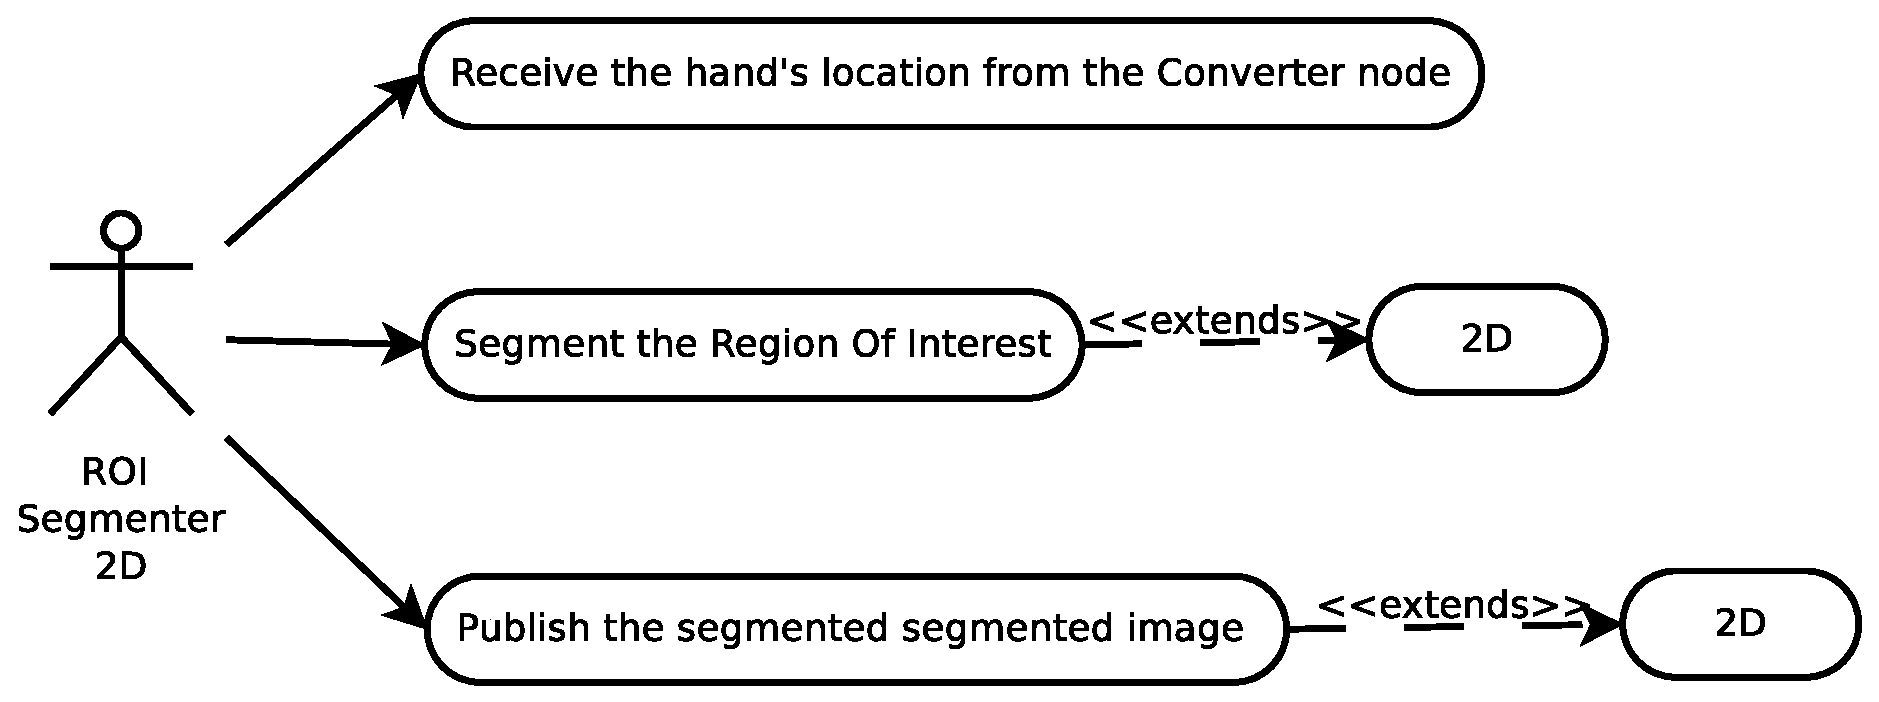
\includegraphics[scale=0.4]{img/diagrams/uc_roi_segmenter_2d.eps}
			\caption[Use case diagram ROI segmenter 2D node]{Use Case diagram of the ROI segmenter 2D node}
		\label{uc_roi2d}
	\end{figure}

%%\newpage

\subsubsection{2D Feature Extractor node}

	This node takes as an input the segmented 2D ROI from the previous nodes and extracts the features. 
	Figure \ref{node_fe2d} shows the Connectivity graph of the node. 

		\begin{figure}[H]
			\begin{center}
			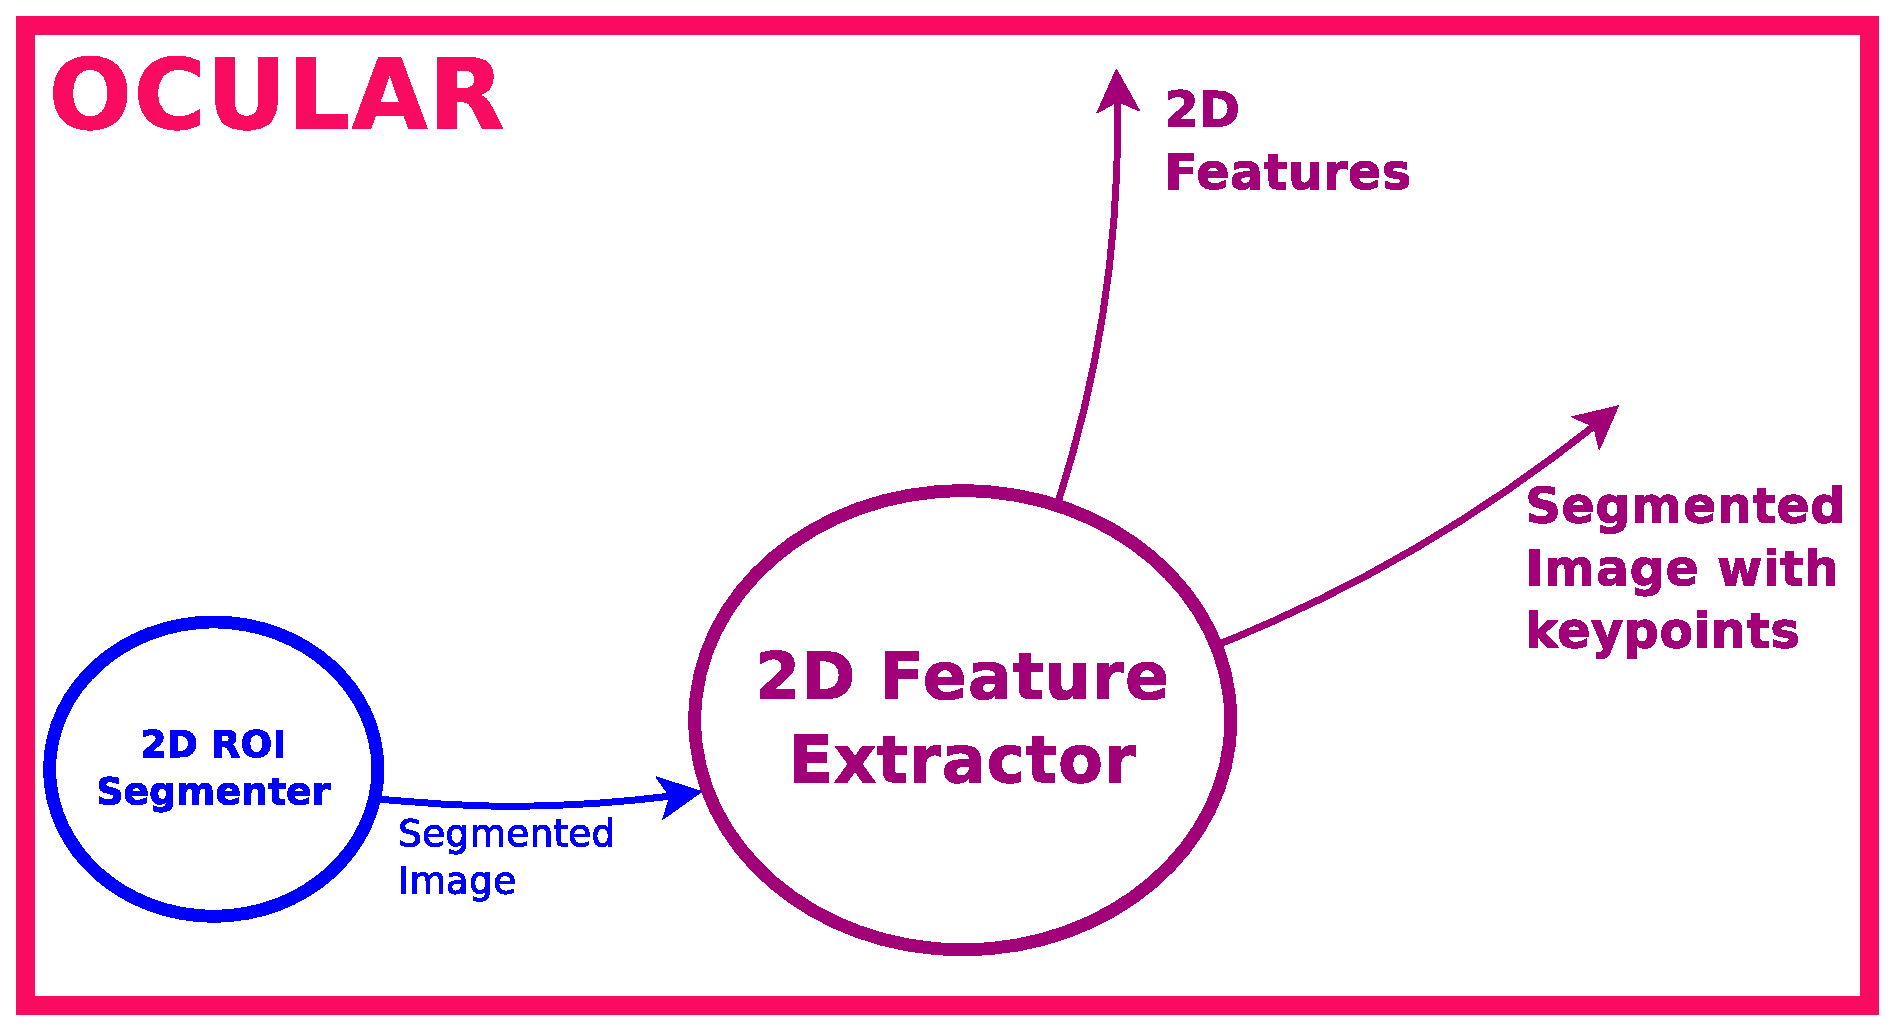
\includegraphics[width=0.5\linewidth]{img/diagrams/node_fe2d.eps}
			\caption[Feature Extractor 2D node I/O]{Connectivity graph of the Feature Extractor 2D node.}		
			\label{node_fe2d}
			\end{center}
		\end{figure}

	There are two output messages of this node, the segmented images with keypoints and the 2D ORB descriptors. 
	The descriptors matrix is the one being used in the rest of the system. 
	The segmented image with the keypoints drawn on it is outputted for debugging and development reasons. 
	\\

	Figure  \ref{uc_fe2d} represents the use case diagram of this node. 
	\begin{figure}[H]
		\centering
			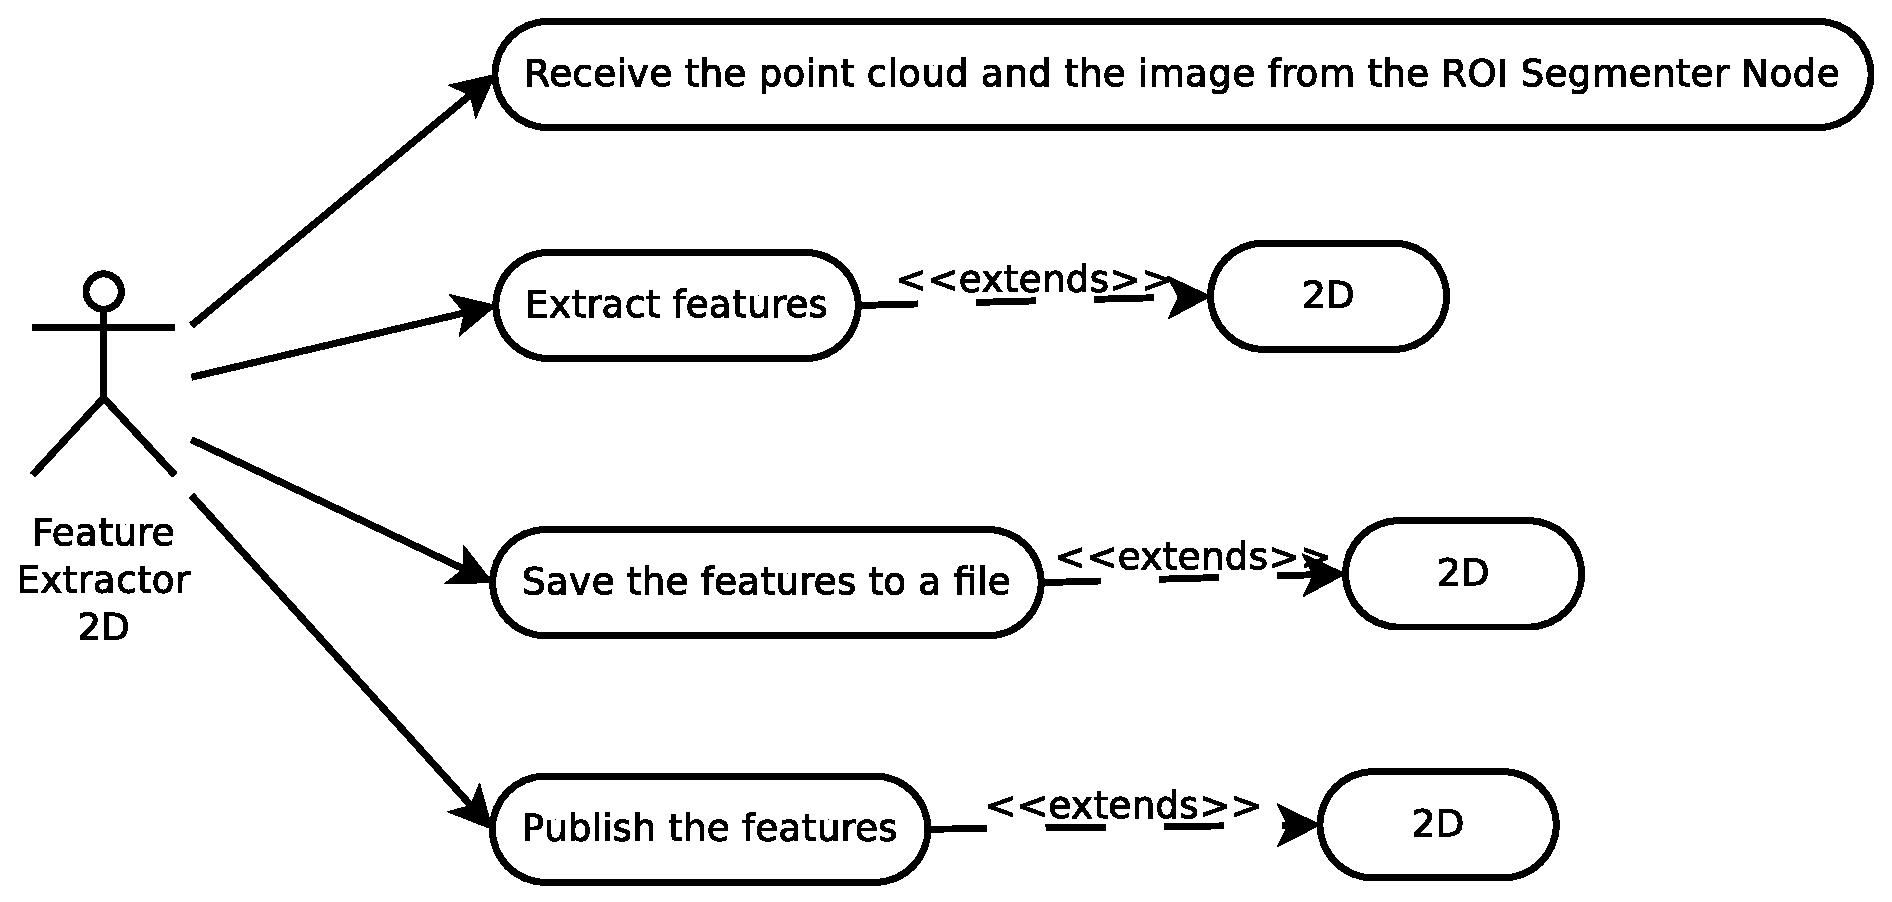
\includegraphics[scale=0.4]{img/diagrams/uc_feature_extractor_2d.eps}
			\caption[Use case diagram Feature Extractor 2D node]{Use Case diagram of the Feature Extractor 2D node}
		\label{uc_fe2d}
	\end{figure}

%%\newpage

\subsubsection{3D Feature Extractor node}

	The input of this node is the segmented point cloud from the ROI Segmenter 3D node (see section \ref{roi_segmenter_3d}. The descriptors are extracted from this information and are published in the output topic. 
	\\
		\begin{figure}[H]
			\begin{center}
			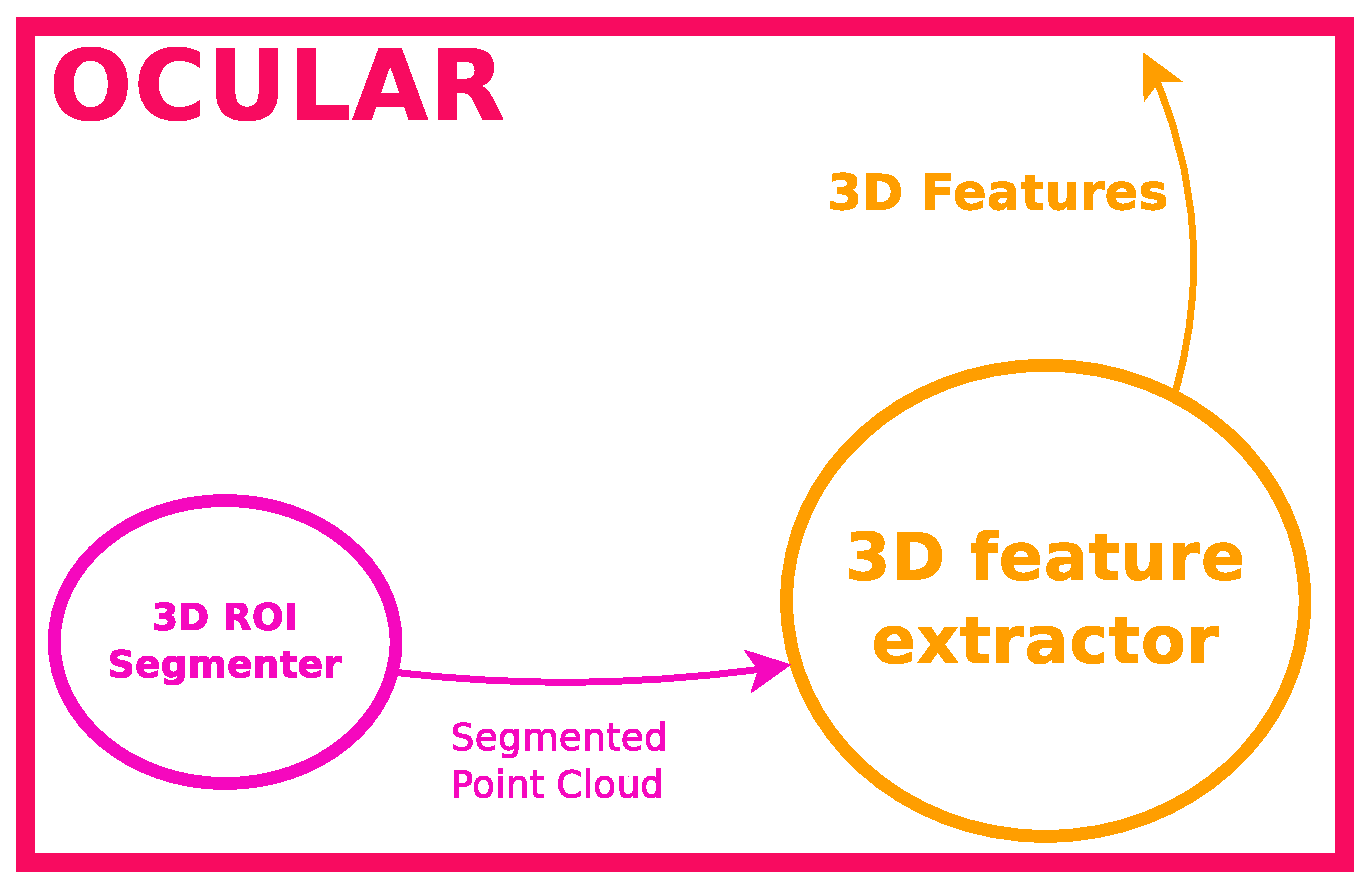
\includegraphics[width=0.5\linewidth]{img/diagrams/node_fe3d.eps}
			\caption[Feature Extractor 3D node I/O]{Connectivity graph of the Feature Extractor 3D node.}		
			\label{node_fe3d}
			\end{center}
		\end{figure}

	Figure \ref{uc_fe3d} shows the use case diagram of the node. 

	\begin{figure}[H]
		\centering
			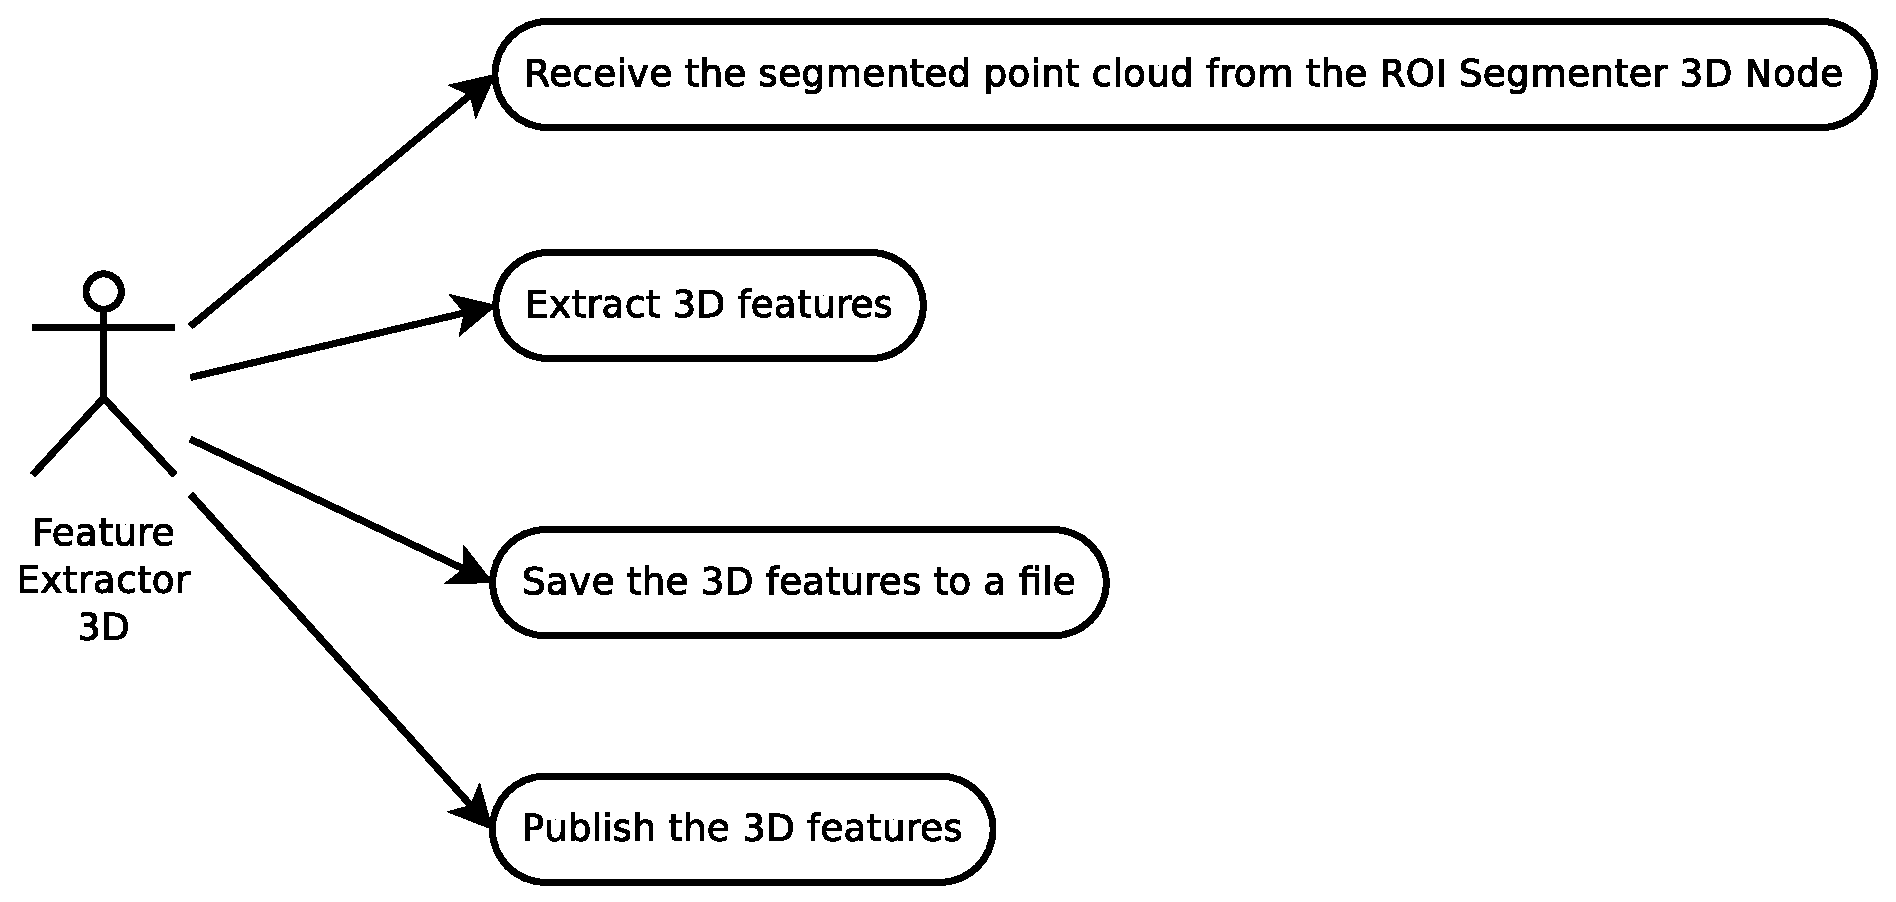
\includegraphics[scale=0.4]{img/diagrams/uc_feature_extractor_3d.eps}
			\caption[Use case diagram Feature Extractor 3D node]{Use Case diagram of the Feature Extractor 3D node}
		\label{uc_fe3d}
	\end{figure}

%%\newpage

\subsubsection{Event Handler node}

	As it was previously stated, in order to interact with the software some gestures were defined. This is the module that detects those gestures and switches accordingly to the corresponding event. This is the node responsible of detecting the different events that can appear in the system. 
	\\
	Figure \ref{node_event} shows the different Connectivity graph of the node. 
		\begin{figure}[H]
			\begin{center}
			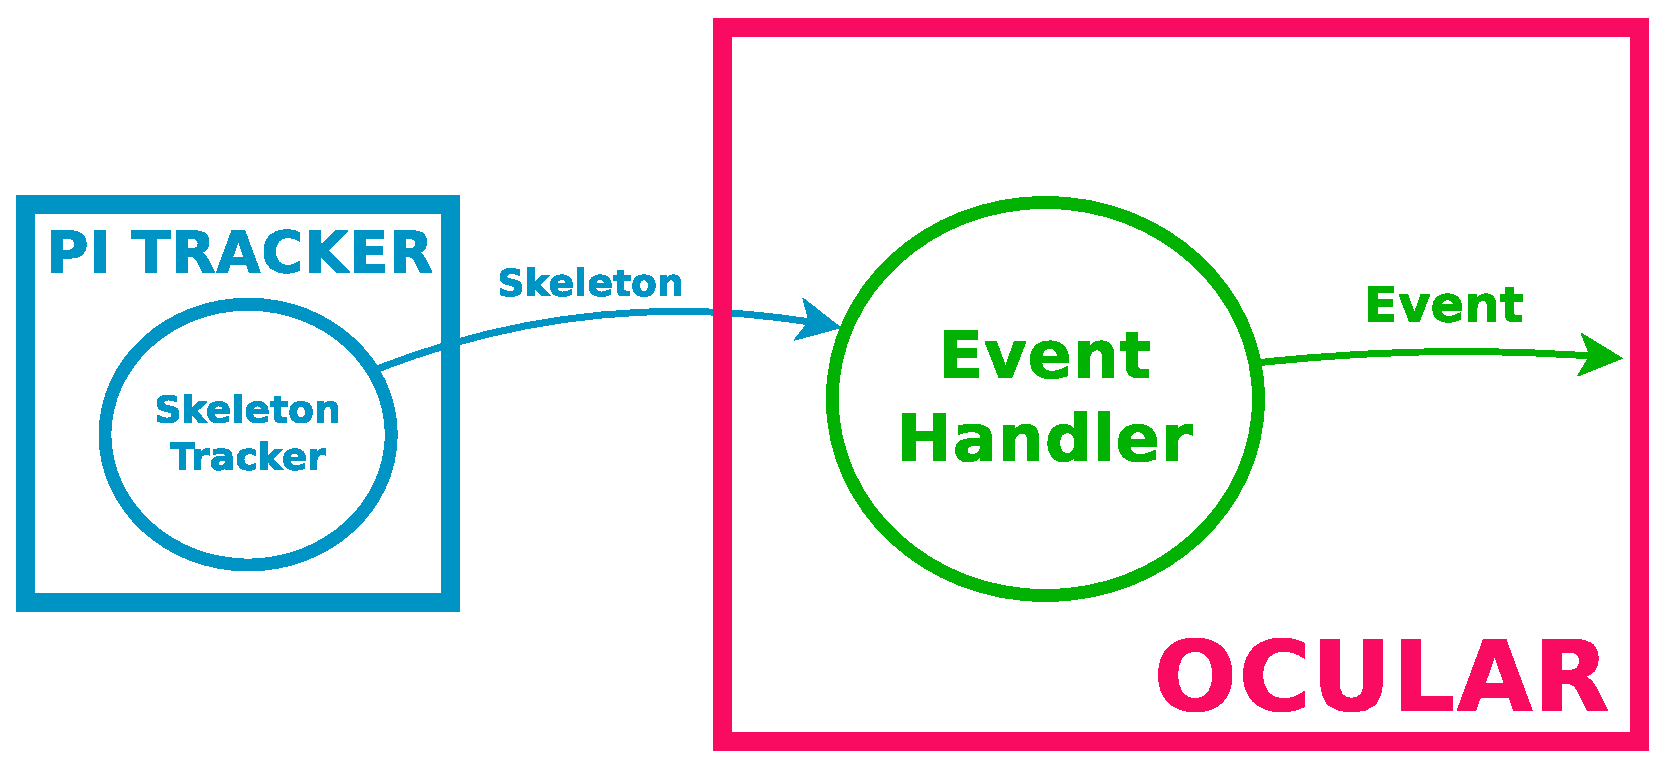
\includegraphics[width=0.5\linewidth]{img/diagrams/node_event.eps}
			\caption[Event Handler 3D node I/O]{Connectivity graph of the Event Handler node.}		
			\label{node_event}
			\end{center}
		\end{figure}
	The input of the system is the skeleton message that is obtained from the third-party package pi\_tracker. This message contains the information of all the joints of the user. The information is screened to detect the height at which each hand is located. The one that is the highest is the one being used in the software. Afterwards, the distance between the body and the chosen hand is computed. When that distance is similar to the distance of the user's arm, the event triggered is "learn". If, otherwise, the hand is located close to the body, the event that is published to the output topic is "recognize". 
	\\

	The distance that triggers the modes is proportional to the distance between the user and the RGB-D sensor in order to obtain a range of use of the software higher. 
	Figure \ref{uc_event} is a diagram with the use case of the node. 
	\begin{figure}[H]
		\centering
			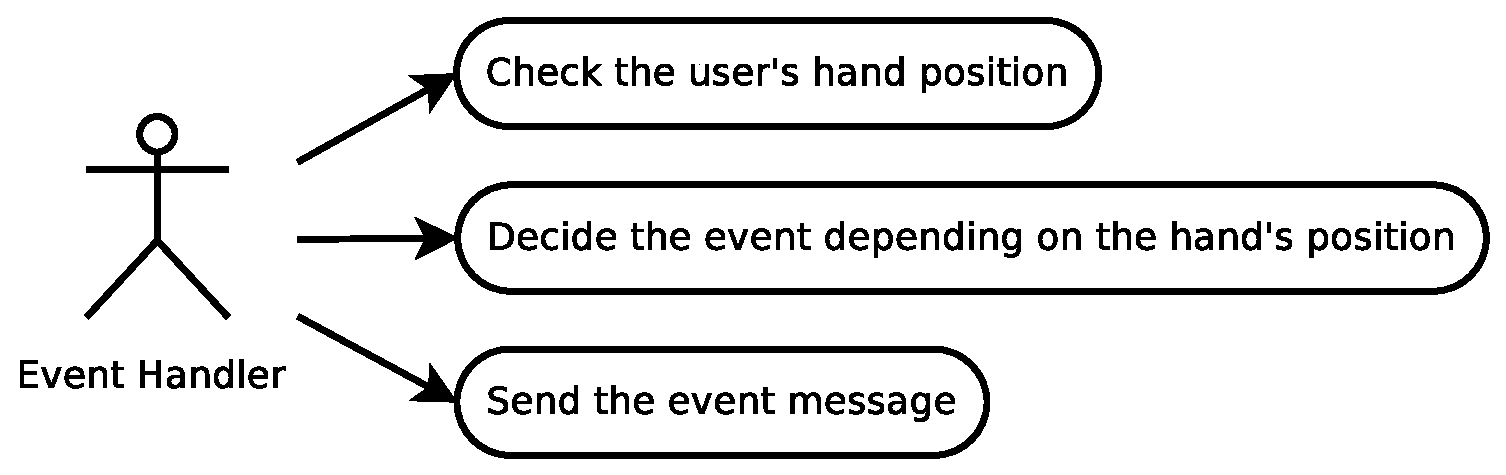
\includegraphics[scale=0.4]{img/diagrams/uc_event_handler.eps}
			\caption[Use case diagram Event Handler node]{Use Case diagram of the Event Handler node}
		\label{uc_event}
	\end{figure}

%%\newpage

\subsubsection{Learner-Recognizer node}
\label{learner_recognizer}

	This node implements the state machine depending on the events recognized by the event handler node. If the event received is "learn", the learning sequence starts. If the event is "recognize", the recognize sequence is triggered. 
	\\

		\begin{figure}[H]
			\begin{center}
			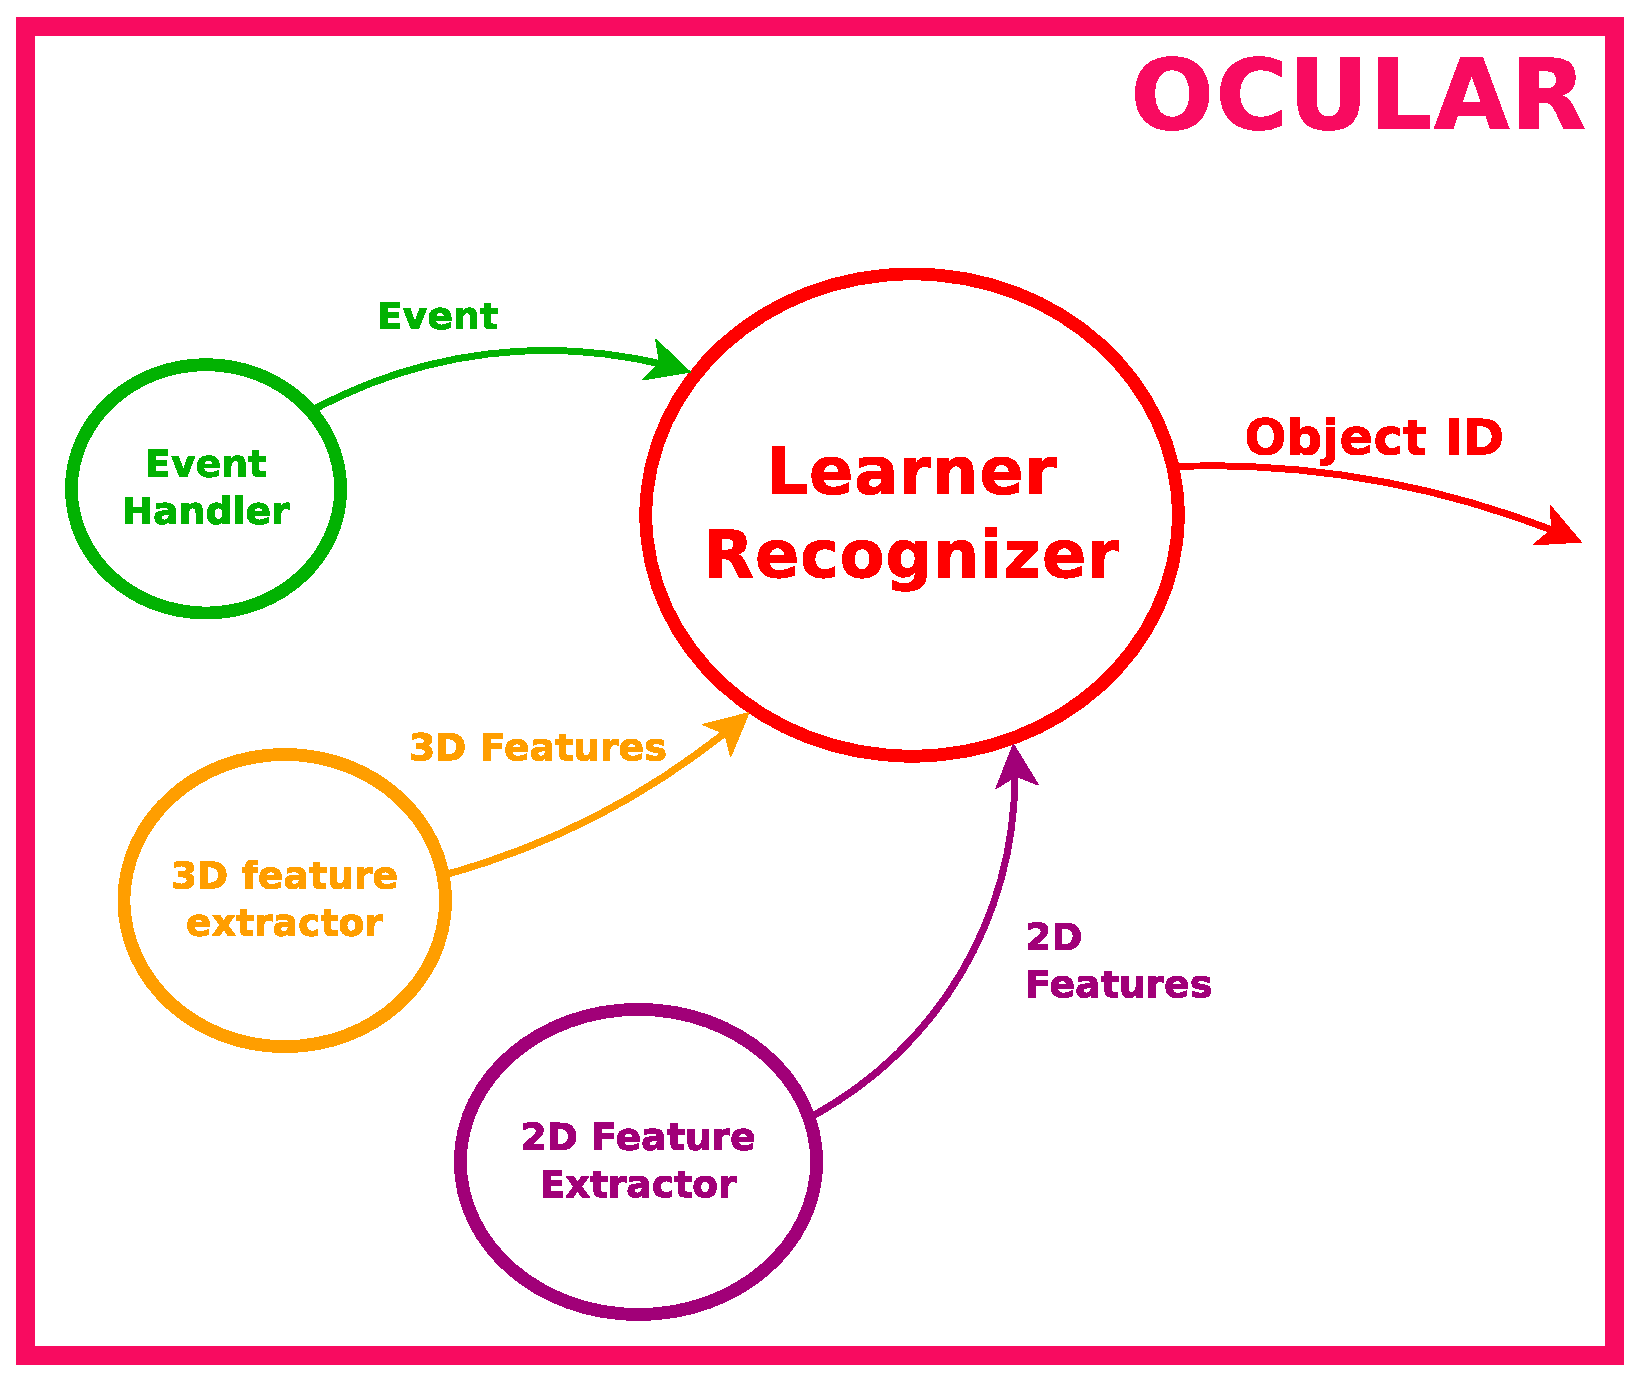
\includegraphics[width=0.5\linewidth]{img/diagrams/node_lr.eps}
			\caption[Learner-Recognizer node I/O]{Connectivity graph of the Learner-Recognizer node.}		
			\end{center}
						\label{node_lr}

		\end{figure}

	The learn sequence consists in obtaining and storing the features both 2D and 3D and waiting a second allowing the user to move the object to capture a new view of it. 
	The dataset extracted is saved to a folder when the software is closed, to prevent possible lags in the runtime of the program. 
	Each view is saved separately. 
	This node loads the files that are still in the saving folder when the program is restarted. 
	\\

	The recognition sequence compares the newly obtained features both 2D and 3D with the ones that are stored in the dataset. 
	Afterwards, the result of the recognition for both types of descriptors are published in the output topic. 
	Figure \ref{uc_learner_recognizer} presents the use case diagram of the node. 

	\begin{figure}[H]
		\centering
			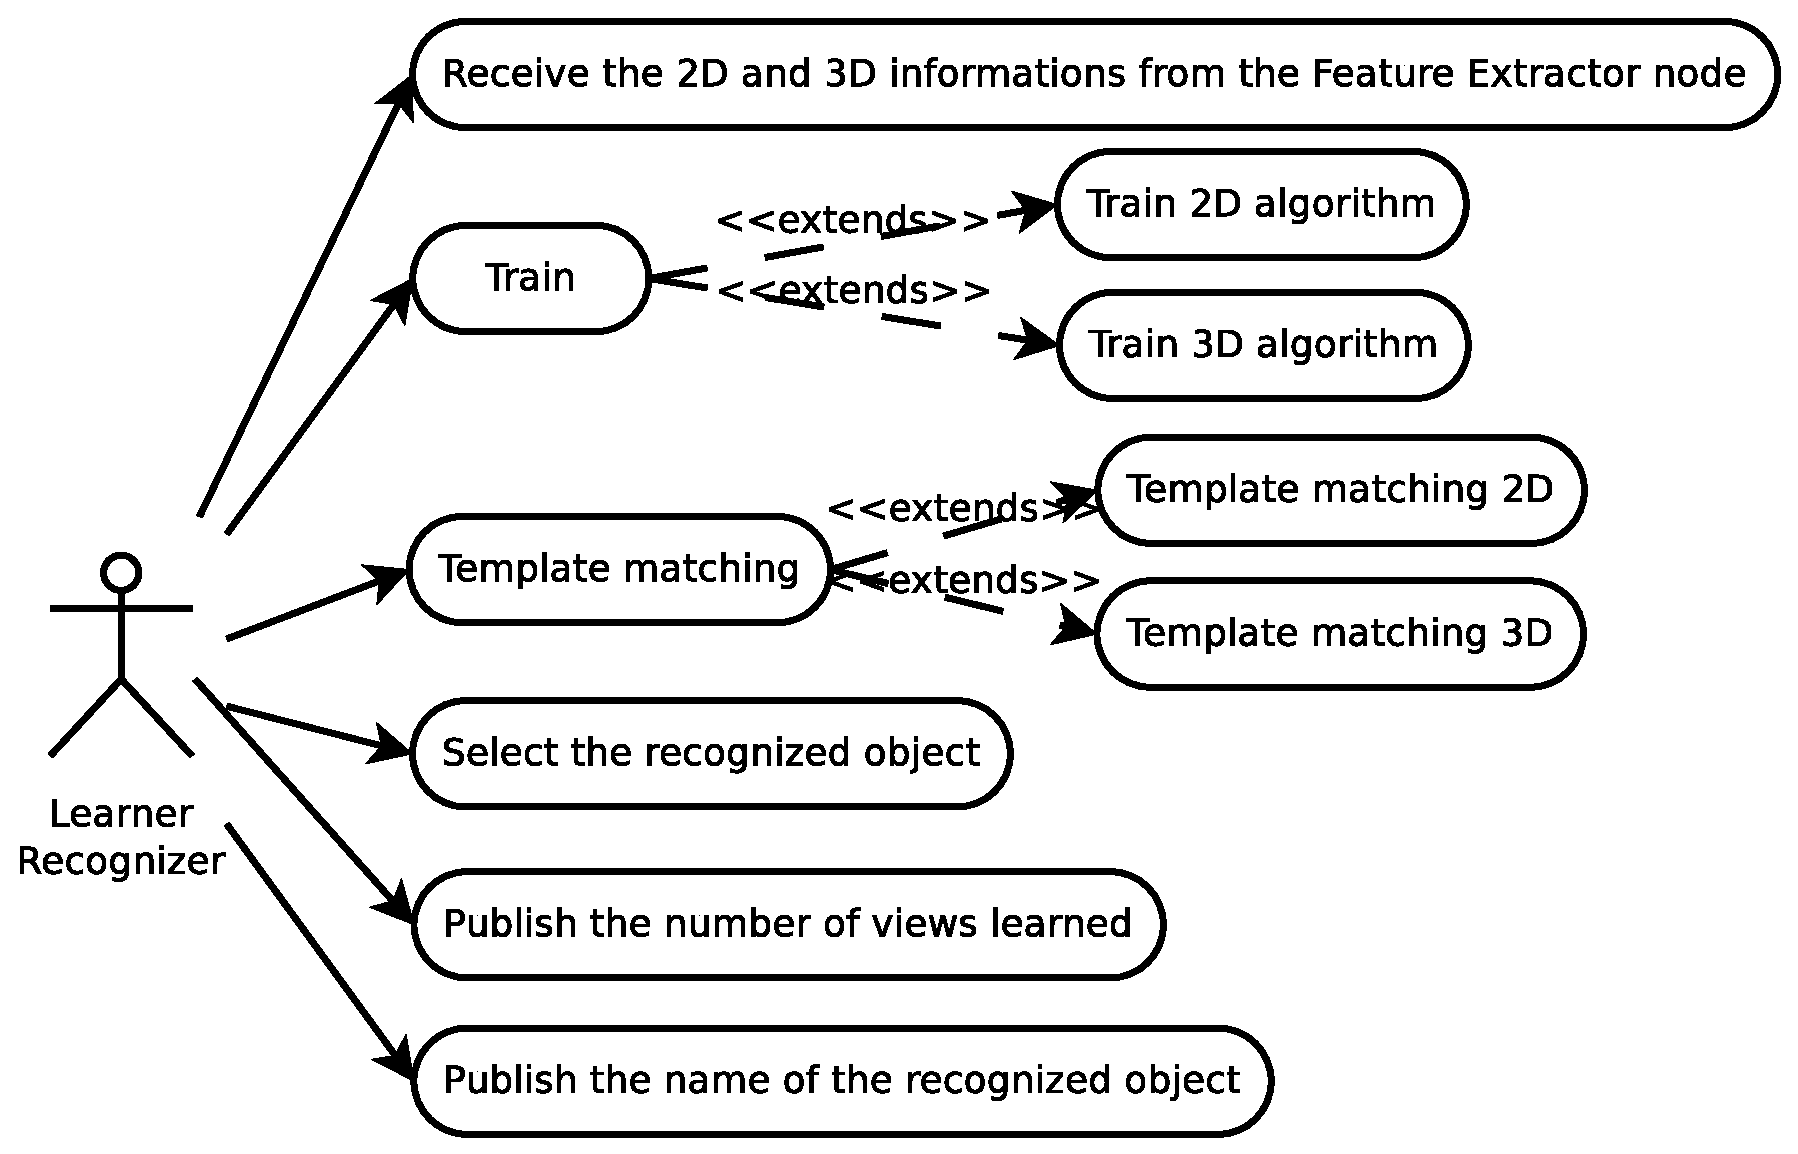
\includegraphics[scale=0.4]{img/diagrams/uc_learner_recognizer.eps}
			\caption[Use case diagram Learner-Recognizer node]{Use Case diagram of the Learner-Recognizer node}
			\label{uc_learner_recognizer}
	\end{figure}

%%\newpage


\subsubsection{System Output node}
\label{last_node}
	This nodes implements a buffer and a decision algorithm. 
	The input of the node is the object ID message from the Learner-Recognizer process as can be seen in figure \ref{node_output}.
	The node stores thirty values of instantaneous object estimations. 
	Since the Kinect runs at 30 frames per second, each second a new final object estimation appears. 
	The output of the node is the final object ID. 


		\begin{figure}[H]
			\begin{center}
			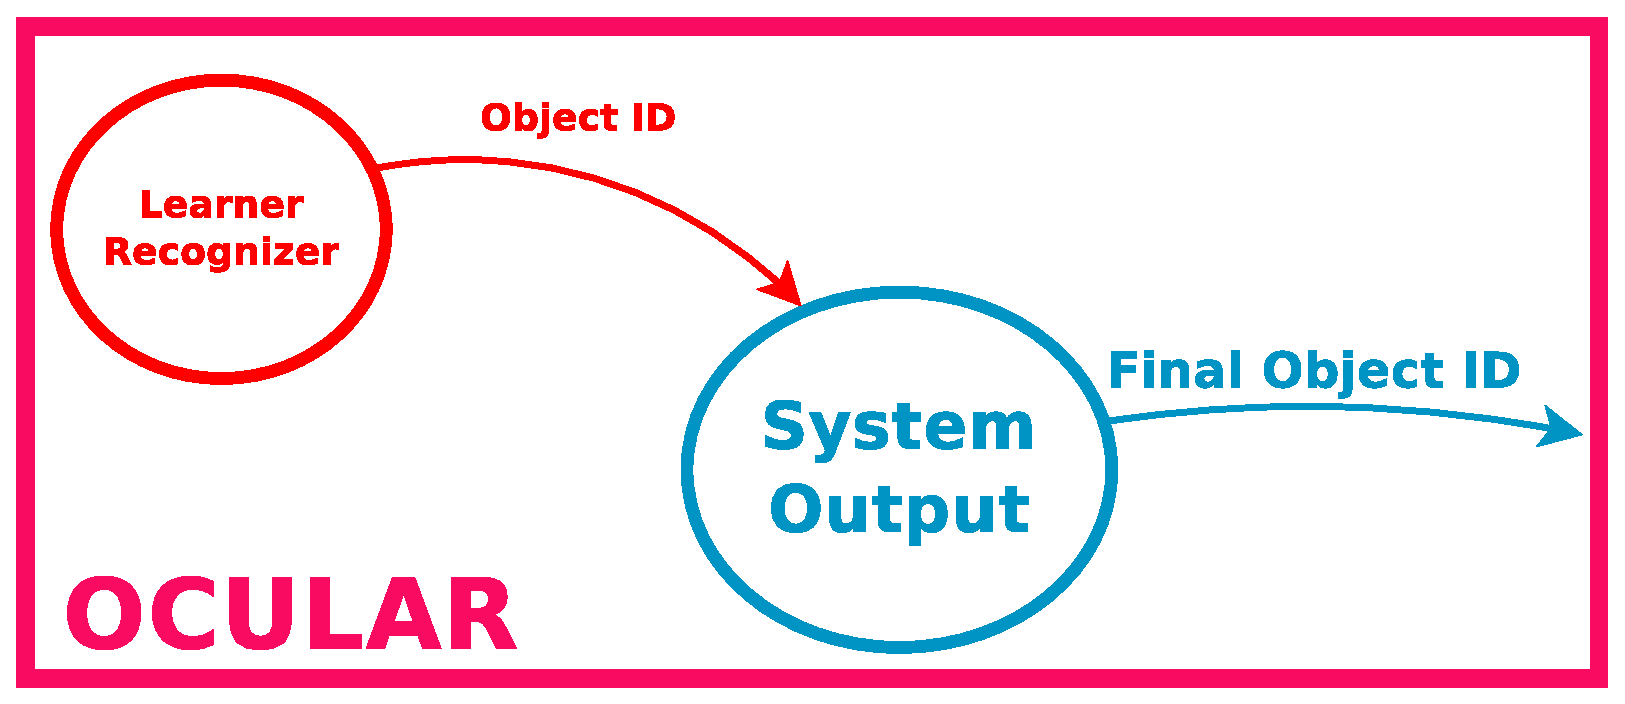
\includegraphics[width=0.5\linewidth]{img/diagrams/node_output.eps}
			\caption[System Output node I/O]{Connectivity graph of the System Output node.}		
			\label{node_output}
			\end{center}
		\end{figure}

	The decision is performed as follows. 
	The input to the algorithm are two vectors containing the 2D and 3D object estimations. 
	The frequency of each class is obtained. 
	Let us represent as $y'_{2D}$ and $y'_{3D}$ the vectors containing in each element the frequency of the object with $object_id = element$. 
	Both informations are combined in one vector called $y'$. 
	\\
	\begin{center}
	$y'=0.6*y'_{2D}+0.4*y'_{3D}$
	\end{center}
	More importance is being given to the 2D estimations since the 2D descriptors are more robust than the 3D ones. 
	The estimated final object id ($Y$) is obtained as the vector element that has the highest value. 
	\\
	\begin{center}
		$Y'= argmax(y')$
	\end{center} 
	This number $Y$ is the output of this whole system. 
	\\
	Figure \ref{uc_output} shows the use case diagram of this node. 

	\begin{figure}[H]
		\centering
			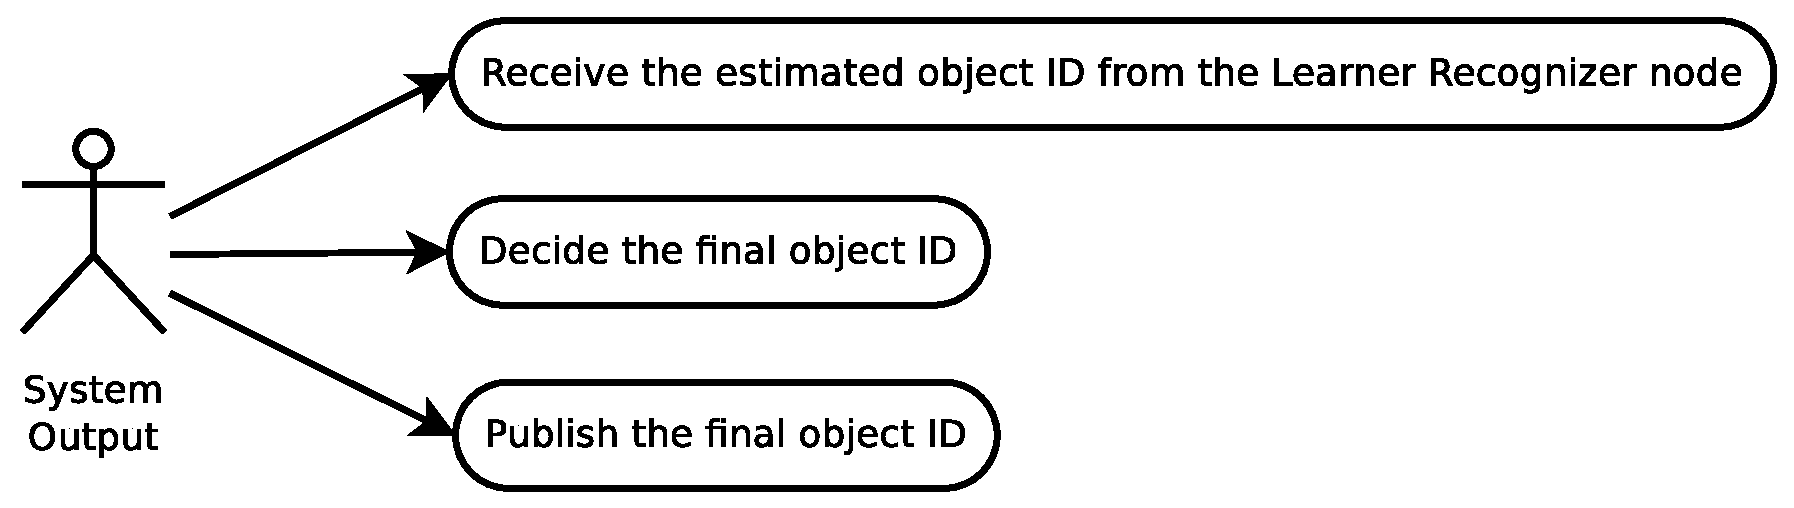
\includegraphics[scale=0.4]{img/diagrams/uc_system_output.eps}
			\caption[Use case diagram System Output node]{Use Case diagram of the System Output node}
			\label{uc_output}
	\end{figure}
 




